%-------------------------------------------------------------------------------
\section{Introduction}
The cortical column is widely regarded as the fundamental processing unit of the neocortex (Mountcastle, 1957).
Under this hypothesis, there is a common microcircuit spanning the depth of the cortex which is repeated across the cortical plane.
As the circuitry of the microcolumn is expected to have structural and functional similarities across the sensory modalities, therefore understanding this generic circuitry of the columnar computation will have far reaching impacts.
However, despite some progress towards understanding knowing the different types of neurons in present in different layers, and the distribution of their most prominent inter-connections, and a structural wiring diagram for the cortical microcircuit, is still unknown.
Furthermore, the functional structure and computation of the microcircuit, which is to say the purpose of the processing in each cortical layer, is also still unknown.
In this paper, we aim to elucidate the functional structure of the cortical layers in \ac{V1} by examining the information contained in population activity at the various layers using \acp{LFP}.

\acp{LFP} are thought to reflect an integration of the membrane depolarisation in the neurons surrounding the electrode location.
The \ac{LFP} captures changes within the dendritic trees of neighbouring neurons as well as the soma.
The low frequency \ac{LFP} (XXXX \si{Hz}) captures slower changes in the population activity, and reflects more of the dendritic level of processing, integrated over a larger region than the high frequency \ac{LFP} (Leski, Linden, Tetzlaff, Pettersen, \& Einevoll, 2013).
%The idea of isolated frequency bands conveying complementary
Since early \ac{EEG} studies, it is has been hypothesized that different frequencies convey complementary information originates with \ac{EEG} studies, but and this has subsequently been extended to the \ac{LFP}.


We previously found that in the macaque \ac{V1} there are two \ac{LFP} frequency bands, \SIrange{1}{8}{Hz} and \SIrange{60}{100}{Hz}, which encode independent information in the macaque \ac{V1} about natural stimuli (Belitski et al., 2008).
In this study we expand the previous study by studying information as a function of cortical depth, and identify one aspect of natural scenes which is encoded differently by the two cortical frequency bands.
We hypothesised the two bands of information are generated through different cortical processes and originate at different locations in the cortex.
In this study we expand the previous study by studying information as a function of cortical depth, and identify one aspect of natural scenes which is encoded differently by the two cortical frequency bands.

Recent work has shown stimulation in \ac{V1} induces gamma activity in \ac{V4} (feedforward), whilst stimulation in \ac{V4} induces alpha oscillations in \ac{V1} (feedback) (van Keroerle et al., 2014).
%-------------------------------------------------------------------------------
\section{Experimental Methods}
\subsection{Ethics Statement}
Data was collected from \ac{V1} in four healthy rhesus monkeys (Macaca mulatta; four males \SIrange{8}{11}{kg}; \SIrange{10}{12}{years}).
All the experimental procedures were approved by the local authorities (Regierungspr\"asidium, Baden-W\"urttemberg, T\"ubingen, Germany; Project Number KY4/09) and were in full compliance with the guidelines of the European Community (EUVD 86/609/EEC) and were in concordance with the recommendation of the Weatherall report for the care and use of non-human primates (Weatherall, 2006).
The animals were group-housed in an enriched environment, under daily veterinarian care.
Weight, food and water intake were carefully monitored on a daily basis.

\subsection{Anesthesia for Neurophysiology Experiments}
The anesthesia protocol for all the experimental procedures have been described previously (Logothetis, Guggenberger, Peled, \& Pauls, 1999; Logothetis, Pauls, Augath, Trinath, \& Oeltermann, 2001).
Briefly, glycopyrrolate (\SI{0.01}{mg.{kg}^{-1}}) and ketamine (\SI{15}{mg.{kg}^{-1}}), were used previous to general anesthesia.
Induction with fentanyl (\SI{3}{mg.{kg}^{-1}}), thiopental (\SI{5}{mg.{kg}^{-1}}) and succinylcholine chloride (\SI{3}{mg.{kg}^{-1}}), animals were intubated and ventilated using a Servo Ventilator 900C (Siemens, Germany) maintaining an end-tidal CO2 of \SIrange{33}{35}{mm.Hg} and oxygen saturation above \SI{95}{\percent}.
The anesthesia was maintained with remifentanil (\SIrange{0.5}{2}{\micro\gram.kg^{-1}.\min}) and mivacurium chloride (\SIrange{2}{6}{mg.kg^{-1}.h}) which ensured no eye movement during electrophygiological recordings.
The anesthetics dosage were established by measuring stress hormones and were selected to ensure unaffected physiological response at normal catecholamine concentrations (Logothetis et al., 1999).
In addition, it has been shown that using remifentanil has no significant effect on the neurovascular and neural activity of brain areas that do not belong to the pain matrix (Goense \& Logothetis, 2008; Zappe, Pfeuffer, Merkle, Logothetis, \& Goense, 2008).
In particular, visual cortex does not bind remifentanil.
We monitored the physiological state of the monkey continuously and kept within normal limits.
Body temperature was tightly maintained at \SIrange{38}{39}{\celsius}.
Throughout the experiment lactate Ringer's (Jonosteril, Fresenius Kabi, Germany) with \SI{2.5}{\percent} glucose was continuously infused at a rate of \SI{10}{ml.kg^{-1}.h^{-1}} in order to maintain an adequate acid-base balance and intravascular volume and blood pressure were maintained by the administration of hydroxyethyl starch as needed (Volulyte, Fresenius Kabi, Germany).


We used anesthetized animals because the preparation allows longer data acquisition times and to associate particular neural events to specific stimulus features without the strong effects of animal cognitive state, including effects of attention and arousal that would introduce additional complication in the interpretation of signals.

\subsection{Visual Stimulation}
A few drops of \SI{1}{\percent} cyclopentolate hydrochloride were used in each eye to achieve mydriasis.
Animals were wearing hard contact lenses (W\"ohlk-Contact-Linsen, Sch\"onkirchen, Germany) to focus the eyes on the stimulus plane.
The visual stimulation in all experimental sessions was presented in the eye with stronger ocular preference of recording sites.
The stimulus was presented using either an in-house custom-built projector (SVGA fibre-optic system with a resolution of 800x600 pixels, a frame rate of \SI{30}{Hz}), or a CRT monitor (Iiyama MA203DT Vision Master Pro 513, frame rate \SI{118}{Hz}) placed at eye level, \SI{50}{\centi\metre} in front of the eye.
We found the same results with both display devices, except that monitor refresh with the \SI{30}{Hz} stimulus induced cortical oscillations at \SI{30}{Hz}.
Since this is the result of using an artificial stimulus with a low refresh rate (a well-known issue at this stimulus frequency), we removed this from the data (see Artefact Removal) and pooled the results across all sessions.
The visual stimulus consisted of high contrast (\SI{100}{\percent}), gamma corrected, fast-moving, colourful movie clips (no soundtrack) from commercially available movies.
Stimulus timings were controlled by a computer running a real-time OS (QNX, Ottawa, Canada).
Stimulus-on periods of \SI{120}{s} (5 sessions; 1 session: \SI{40}{s}) were interleaved with stimulus-off periods (isoluminant grey screen) of \SI{30}{s}.


\subsection{Neurophysiology Data Collection and Analysis}
The electrophysiological recordings were performed by doing a small skull trepanation, after which the dura was visualized with a microscope (Zeiss Opmi MDU/S5, Germany) and carefully dissected.
The electrodes were slowly advanced into the visual areas under visual and auditory guidance using manual micromanipulator (Narashige Group, Japan).
Electrodes consisted of laminar probes (NeuroNexus Technologies, Ann Arbor, USA).
These electrodes contained 16 contacts on a single shank \SI{3}{\milli\metre} long and \SI{150}{\micro\metre} thick.
The electrode sites were spaced at \SI{150}{\micro\metre} apart, with a recording area of \SI{413}{\micro\metre^2} each.
We used a flattened \ac{Ag} wire, which was positioned under the skin, as reference electrode (Murayama et al., 2010).
The recording access was filed with a mixture of \SI{0.6}{\percent} agar dissolved in \ac{NaCl} \SI{0.9}{\percent}, pH 7.4 solution which guaranteed good electrical connection between the ground contact and the animal (Oeltermann, Augath, \& Logothetis, 2007).
The impedance of the contact points was always measured during the experiments and ranged from \SIrange{480}{800}{\kilo\ohm}.
The signals were amplified and filtered into a broadband of \SIrange{1}{8000}{Hz} (Alpha-Omega Engineering, Nazareth, Israel) and then digitized at \SI{20.833}{\kilo\Hz} with 16 bit resolution (PCI-6052E; National Instruments, Austin, TX).

\subsection{Luminosity Function}
In order to best approximate the luminosity perceived by macaques, we relied on analogies with the human visual system.
Research with humans suggest the luminosity function is linearly related to the long (L) and medium (M) cone activation, and independent of the short (S) cone activation (Stockman, Jagle, Pirzer, \& Sharpe, 2008).
Furthermore, the weighting of L and M activations towards perceived luminance is believed to be similar to the L:M ratio in the individual (Stockman et al., 2008).
Old world monkeys such as macaques have an L:M ratio which is approximately 1:1 (Dobkins, Thiele, \& Albright, 2000), so we assumed a luminosity function equally weighed between the L and M cone activations,  $Y=L+M$.
The \SI{10}{\degree} cone fundamentals of Stockman \& Sharpe (2000) were used since the cone fundamentals of old world monkeys are known to be very similar to humans (Dobkins et al., 2000).
By taking the product of the emission spectra for pure red, green and blue with the luminosity function, integrating over wavelength and normalising, we obtained the following equations for relative luminance in terms of pixel intensity for the two devices used in the experiment .

\begin{align*}
    Y_{\text{projector}} &= 0.2171 \cdot R + 0.6531 \cdot G + 0.1298 \cdot B\\
    Y_{\text{CRT}}       &= 0.1487 \cdot R + 0.6822 \cdot G + 0.1691 \cdot B
\end{align*}

\subsection{Artefact Removal}
An artefact removal procedure was performed to reduce the effects of line noise (one session) and monitor refresh (the three sessions with \SI{30}{Hz} stimulus).
Artefact frequencies were identified by large, localised peaks in the power spectral density, which was computed with the periodogram method (see Supplementary Table 1).
In each case, the average artefact waveform was found and subtracted from the recorded signal.
To correct for phase shifts of the artefact, the averaging and subsequent subtraction were performed in blocks of 50 artefact periods with a phase chosen to maximise the cross-covariance of the signal with the artefact waveform.

\subsection{Current Source Density}
The \ac{CSD} was computed using the inverse \ac{CSD} method (Pettersen, Devor, Ulbert, Dale, \& Einevoll, 2006).
To compute this, we used a $\delta$-source model of local field generation with a diameter of \SI{500}{\micro\metre}, chosen to correspond to the effective size of columnar activity (Horton \& Adams, 2005; Lund, Angelucci, \& Bressloff, 2003).
Since this method requires an even spacing between voltage measurements, gaps caused by faulty recording contacts in the electrode were filled in with a local average (W\'ojcik \& Leski, 2010).
A homogeneous cortical conductivity of \SI{0.4}{\siemens\per\metre} was assumed (Logothetis, Kayser, \& Oeltermann, 2007).
The agar solution placed on top of the recording access point had an \ac{NaCl} concentration of \SI{9}{\mg\per\mL}, and the conductivity of this was estimated to be \SI{2.2}{\siemens\per\metre} (Kandadai, Raymond, \& Shaw, 2012).
The \ac{CSD} was spatially smoothed with a three-point Hamming filter (add ref that justifies this smoothing).

\subsection{Multiunit Activity}
Fig.~\ref{fig:lam_1}: \ac{MUA} was calculated by band-passing the voltage recording between 900 and \SI{3000}{Hz} with a zero-phase sixth-order Butterworth filter, taking the absolute value, applying a \SI{300}{Hz} low pass third-order Butterworth filter, and then downsampling.
This yields a smoothed spike rate, analogous to a population firing rate.

Fig.~\ref{fig:lam_3}: \ac{MUA} was calculated by downsampling by a factor of 3, band-passing the voltage recording between \SIrange{900}{3000}{Hz} with a zero-phase sixth-order Butterworth filter, taking the absolute value, downsampling by a further factor of 12.

\subsection{Receptive Field Locations}
The spatial \acp{RF} were found by reverse correlating the \ac{MUA} and the pixel-by-pixel Z-scored frame-by-frame difference in luminance with a fixed lag of \SI{66.7}{ms}.
The rate of change in luminance was used because it is known to correlate well with thalamic drive.
For each session, the \ac{RF} centre was located using the average of the reverse correlation across all cortical channels.

\subsection{Identification of Cortical Laminae}
Depth calibration of the electrode was performed by considering the spikes and \ac{CSD} induced by both the onset of the movie and by \SI{100}{ms} full-screen flashes (\SI{6}{s} flash interval).
From the measured potentials, we determined the \ac{CSD} and spike densities.
Spikes were detected by high pass filtering the raw signal above \SI{500}{Hz} with a zero-phase eighth-order Butterworth filter, and classifying any points more than 3.5 standard deviations above the mean signal during pre- and post-stimulus periods as a spike, with a minimum inter-spike-interval of \SI{1}{ms}.
The majority of thalamic afferents in \ac{V1} stimulate \ac{L4} (indirectly: see Hansen et al. (2012)), with the first cortical response manifesting at layer 4C$\alpha$ (E. M. Callaway, 1998), resulting in an initial current sink and first burst of spiking activity located here.
For each recording session, we found the contact exhibiting the first spiking and \ac{CSD} response, the centre of the most responsive region, and the centre of the first \ac{CSD} sink for both the movie onset and flash evoked activity.
We took the average of these 8 locations and identified the closest electrode contact as the location of layer 4C$\alpha$.
We estimated the laminar location of the rest of the recording depths by cross-referencing literature describing average thickness of cortical laminae in Macaca mulatta, area 17, (Lund, 1973).
From this, the cortical depth was divided into 3 broad regions: supragranular (SG; layers 1--3), granular (G; layer 4), and infragranular (IG; layers 5--6).
High-resolution \ac{MRI} scans of two of the animals were used to determine their cortical thickness at the recording location (see Supplementary Materials).

\subsection{Identification of cortical laminae}
To identify the depth of each contact, we measured the potential evoked in response to the onset of the movie clip, and in response to full-screen maximum-luminance \SI{100}{ms} flash stimuli with a \SI{6}{s} interval.
From the measured potentials, we identified the boundary between the granular (G; layer 4) and infragranular (IG; layers 5--6) regions as the source/sink reversal in the evoked current source density (\ac{CSD}; see Experimental Procedures and Supplementary Materials).
We estimated the location of the boundary between the granular and supragranular (SG; layers 1--3) regions by cross-referencing literature describing average thickness of cortical laminae in Macaca mulatta, area 17 (Lund, 1973).

\subsection{Power as a function of depth and frequency}
To compute power and information as a function of temporal frequency, the cortical data (\ac{LFP} and \ac{CSD}) were filtered in a series of bands each with a fractional bandwidth of \SI{50}{\percent}, because cortical power falls off rapidly with frequency in a \nicefrac{1}{f} relationship.
Each successive band begins and ends with frequencies 1.291 times higher than the last, so that each band has \SI{0}{\percent} overlap with bands further away than its immediate neighbours and a \SI{44}{\percent} and \SI{56}{\percent} overlap with its preceding and succeeding bands respectively.
The data was filtered with a zero-phase sixth-order Butterworth filter, after which the instantaneous power was estimated by taking the squared absolute value of the Hilbert transform.
The power in each band was integrated over a series of \SI{50}{ms} windows, centred at the time of each frame change in the movie (once every \SI{33}{ms}, leading to a \SI{50}{\percent} overlap of neighbouring windows).
The power in the \SIrange{4}{16}{Hz} and \SIrange{60}{170}{Hz} bands was computed similarly.
Fig.~\ref{fig:lam_3}A--B are plotted with power values averaged over all windows and trials, then expressed in decibels relative to the average power \SIrange{1.5}{248}{Hz} (estimated by summing the power in alternate bands).
Throughout Figures 3 and S3, datapoints are shown at the band centres.

\subsection{Information as a function of depth and frequency}
Power in each band was computed as above, then for each frequency band and depth we took a 10-bin histogram of the power across all the 50ms windows for all repetitions.
The bin edges were chosen such that \SI{10}{\percent} of the distribution fell into each bin, and the identity of which bin the window was allocated into was taken to be its ``stimulus''.
We found the mutual information between the response and which frame was on screen at that time --- the ``stimulus'' --- by computing the Shannon information using the information breakdown toolbox (Magri, Whittingstall, Singh, Logothetis, \& Panzeri, 2009).
Bias due to undersampling was corrected for using the \ac{PT} method (Treves \& Panzeri, 1995).
Each information calculation was also bootstrapped 20 times with a randomly shuffled mapping of stimulus to response (also bias-corrected).
To ensure the amount of information was statistically significant, we checked each information estimate exceeded the bootstrap mean by more than 3 standard deviations of the bootstrap values.
The bootstrap mean was then subtracted from the estimated information, to counter any residual bias.

\subsection{Cortical Distribution of Power}
For each session, the distribution of power across the cortical depth (2A--B right-hand insets) was determined by normalising the power at each depth by the summed power across all cortical depths for that band.
We then took an average across sessions, weighted by the number of cortical recording sites in each session to prevent faulty (omitted) electrode contact sites from distorting the result.

\subsection{Information Redundancy}
Information redundancy was computed with the same stimuli windows as used in the information calculations.
Let  $S$ denote the set of stimuli, and let  $X$ and  $Y$ each be the set of powers during each stimulus in one of the frequency bands at a particular depth.
The information in each  $I\left(X;S\right)$ and  $I(Y;S)$ was computed in the same manner as above.
The information in the joint distribution  $I(\left\{X,Y\right\};S)$ was computed by considering each combination of the binned  $X$ and  $Y$ as a different response, yielding a total of 100 different responses for  $\{X,Y\}$.

The relative redundancy is then defined as
\begin{equation*}
\mathit{Redundancy}=\frac{I\left(X;S\right)+I\left(Y;S\right)-I\left(\left\{X,Y\right\};S\right)}{I\left(\left\{X,Y\right\};S\right)}
\end{equation*}
and was computed using the information breakdown toolbox (Magri et al., 2009).


\subsection{Information at about Spatial Components}
The method to find the change in luminance in each spatial frequency band is illustrated in Fig.~\ref{fig:lam_4}.
First, we took the 2D fast-Fourier transform of a 224px square from the movie.
A fourth-order Butterworth filter with a width of one octave was applied using a mask in the Fourier domain, and the result was projected back to the spatial domain.
We then took the pixel-wise difference between each spatially filtered pair of consecutive frames.
To provide a measure of the amount of change in luminance at this spatial resolution, we took the absolute amount of change in each pixel and summed this within a \SI{2}{\degree} diameter circular window centred at the receptive field location.

Applying this to the entire movie provided a temporal sequence of luminance changes in each spatial range.
Similar to before, we took a 10-bin histogram and took the identity the bin in which each luminance change fell to be the ``stimulus''.
The mutual information between this stimulus and the neural response --- the power within \SIrange{4}{16}{Hz} and \SIrange{60}{170}{Hz} frequency bands --- was computed with a 67ms lag between stimulus and response.

\subsection{Information about Fine and Coarse Luminance Changes}
Coarse and fine luminance changes in the stimulus were isolated in the same manner as the spatial components above, but using a low-pass (\SI{<0.3}{\cpd}) and high-pass (\SI{>1}{\cpd}) fourth-order Butterworth filter respectively.
For both the \SIrange{4}{16}{Hz} and \SIrange{6}{170}{Hz} \ac{CSD} powers, we computed the correlation and mutual information with the coarse and fine luminance changes, and averaged across sessions.

\subsection{Information lag between granular and infragranular regions}
The information about fine and coarse stimuli contained in \SIrange{4}{16}{Hz} and \SIrange{60}{170}{Hz} neural frequency bands was computed as a function of the lag between stimulus and response, in steps of 1.73ms.
For each cortical recording depth, we found response lag at which the information was at its maximum.
For each session, the response peak-lag was averaged across the three electrode contacts in \ac{IG} and also averaged across the three electrodes in \ac{G}.
A paired t-test was performed across all 6 sessions to test whether the \ac{G} information peaked with a shorter lag than the \ac{IG} information.

\subsection{Cross-Frequency Phase-Amplitude Coupling}
Strength of cross-frequency coupling was measured using the Modulation Index (Tort, Komorowski, Eichenbaum, \& Kopell, 2010).
\ac{CSD} data was filtered for two bands, \SIrange{4}{16}{Hz} and \SIrange{60}{170}{Hz}, using a zero-phase sixth-order Butterworth filter, and the instantaneous phase of \SIrange{4}{16}{Hz} and envelope amplitude of \SIrange{60}{170}{Hz} were each estimated using a Hilbert transform.
We took a histogram of the \SIrange{4}{16}{Hz} phase datapoints with 16 bins each of width $\nicefrac{\pi}{8}$ radians, and took the average of the \SIrange{60}{170}{Hz} amplitudes simultaneous with the phase datapoints in each bin.
This provides a distribution of amplitude at one depth as a function of phase at another.
The Modulation Index is then the normalised Kullback-Leibler divergence of this distribution from a uniform distribution.

%-------------------------------------------------------------------------------
\section{Results}
Four anesthetized monkeys (Macaca mulatta) were presented with a Hollywood movie clip, repeated 40--150 times, whilst we recorded neural activity in the \ac{V1} with a multicontact laminar electrode.
Each electrode housed 16 equally spaced (150\hspace{0.2em}$\mu$m) contacts spanning a total depth of 2250\hspace{0.2em}$\mu$m, and was inserted perpendicular to the cortical surface (Fig.~\ref{fig:lam_1}A).
We identified the depth of each probe using the \ac{CSD}, and identified \ac{G}, \ac{SG}, and \ac{IG} cortical regions based on literature (see Experimental Methods for details).
We performed reverse correlation between the rate of change of luminance for each pixel in the movie and the \ac{MUA} at each contact site to find the spatial-\ac{RF} (Fig.~\ref{fig:lam_1}B).
The \ac{RF} locations did not vary with depth, indicating that all electrode contacts were recording from the same cortical column.

\begin{figure}[htbp]
\centering 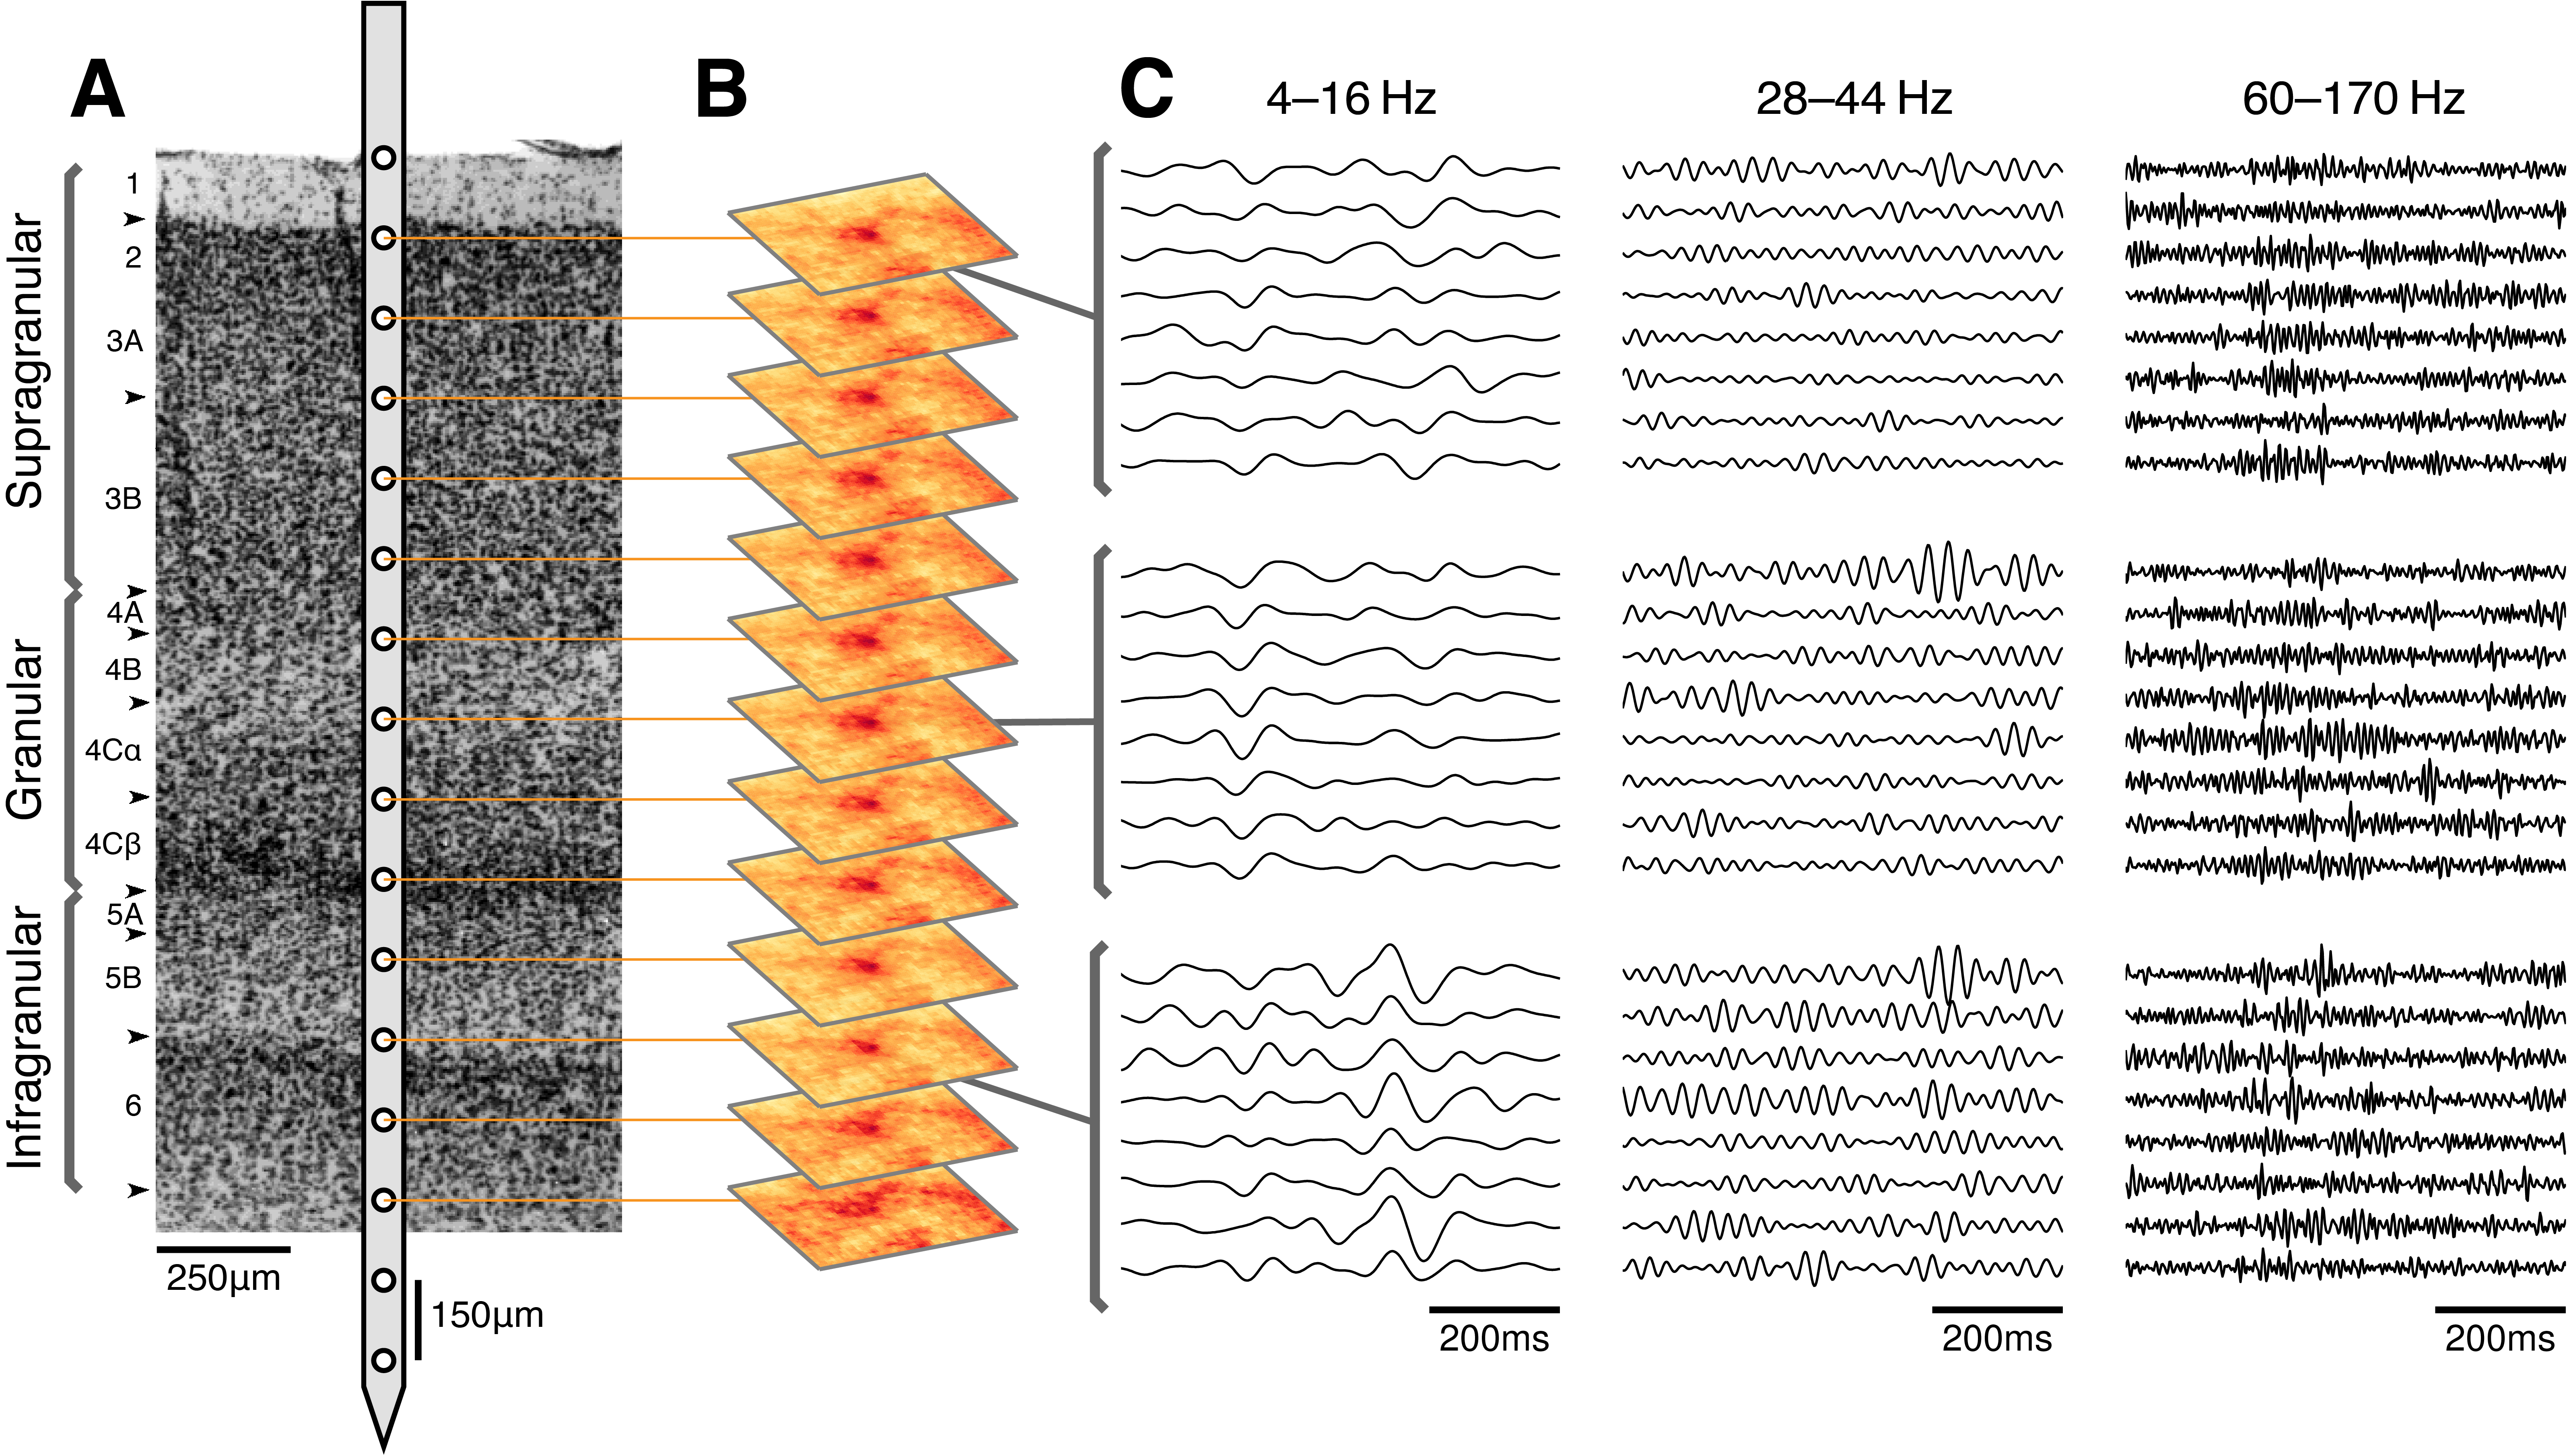
\includegraphics[width=\columnwidth]{fig1}
%
\caption{%
\textit{Overview of data collection and example data.}
A: Illustration of experimental recording setup, showing approximate locations 
of electrode contacts in relation to a Nissl-stained section of macaque \ac{V1} 
cortex.
Boundaries between cortical laminae are indicated with arrowheads.
(Stain reproduced from Tyler et al. 1998, with permission.) (Note: Electrode 
width is not to scale.)
B: Receptive field locations were consistent across the 
cortical depth.
Location of receptive field for each cortical recording site 
was identified by reverse 
correlating the \ac{MUA} with the luminance changes of each 
pixel in the movie (session E07nm1).
C: Example \ac{CSD} traces from simultaneous recordings at three cortical depths for eight 
repetitions of a movie fragment (session H05nm7).
The data are split into three temporal frequency bands (\SIrange{4}{16}{Hz}, 28-44Hz and \SIrange{6}{170}{Hz}, see Methods).
}%
\label{fig:lam_1}
%
\end{figure}

\subsection{Distribution of information across depth and frequency}
Fig.~\ref{fig:lam_1}C shows, at three cortical depths, \ac{CSD} traces from eight example trials during a portion of the stimulus.
The traces have been filtered within three frequency bands: \SIrange{4}{16}{Hz}, \SI{28}{44}{Hz} and \SIrange{60}{170}{Hz}.
One can observe that the low-frequency activity repeats across trials for the \ac{G} and \ac{IG} depths.
Activity in the \SI{28}{44}{Hz} range is inconsistent at all depths, and does not seem to be stimulus modulated.
The envelope amplitude of the \SIrange{60}{170}{Hz} band is also consistent across trials, most clearly for the \ac{SG} depth.
The mutual information We quantified these observations by computing the amount of information about the movie contained in the neural activity.

\begin{figure}[htbp]
\centering 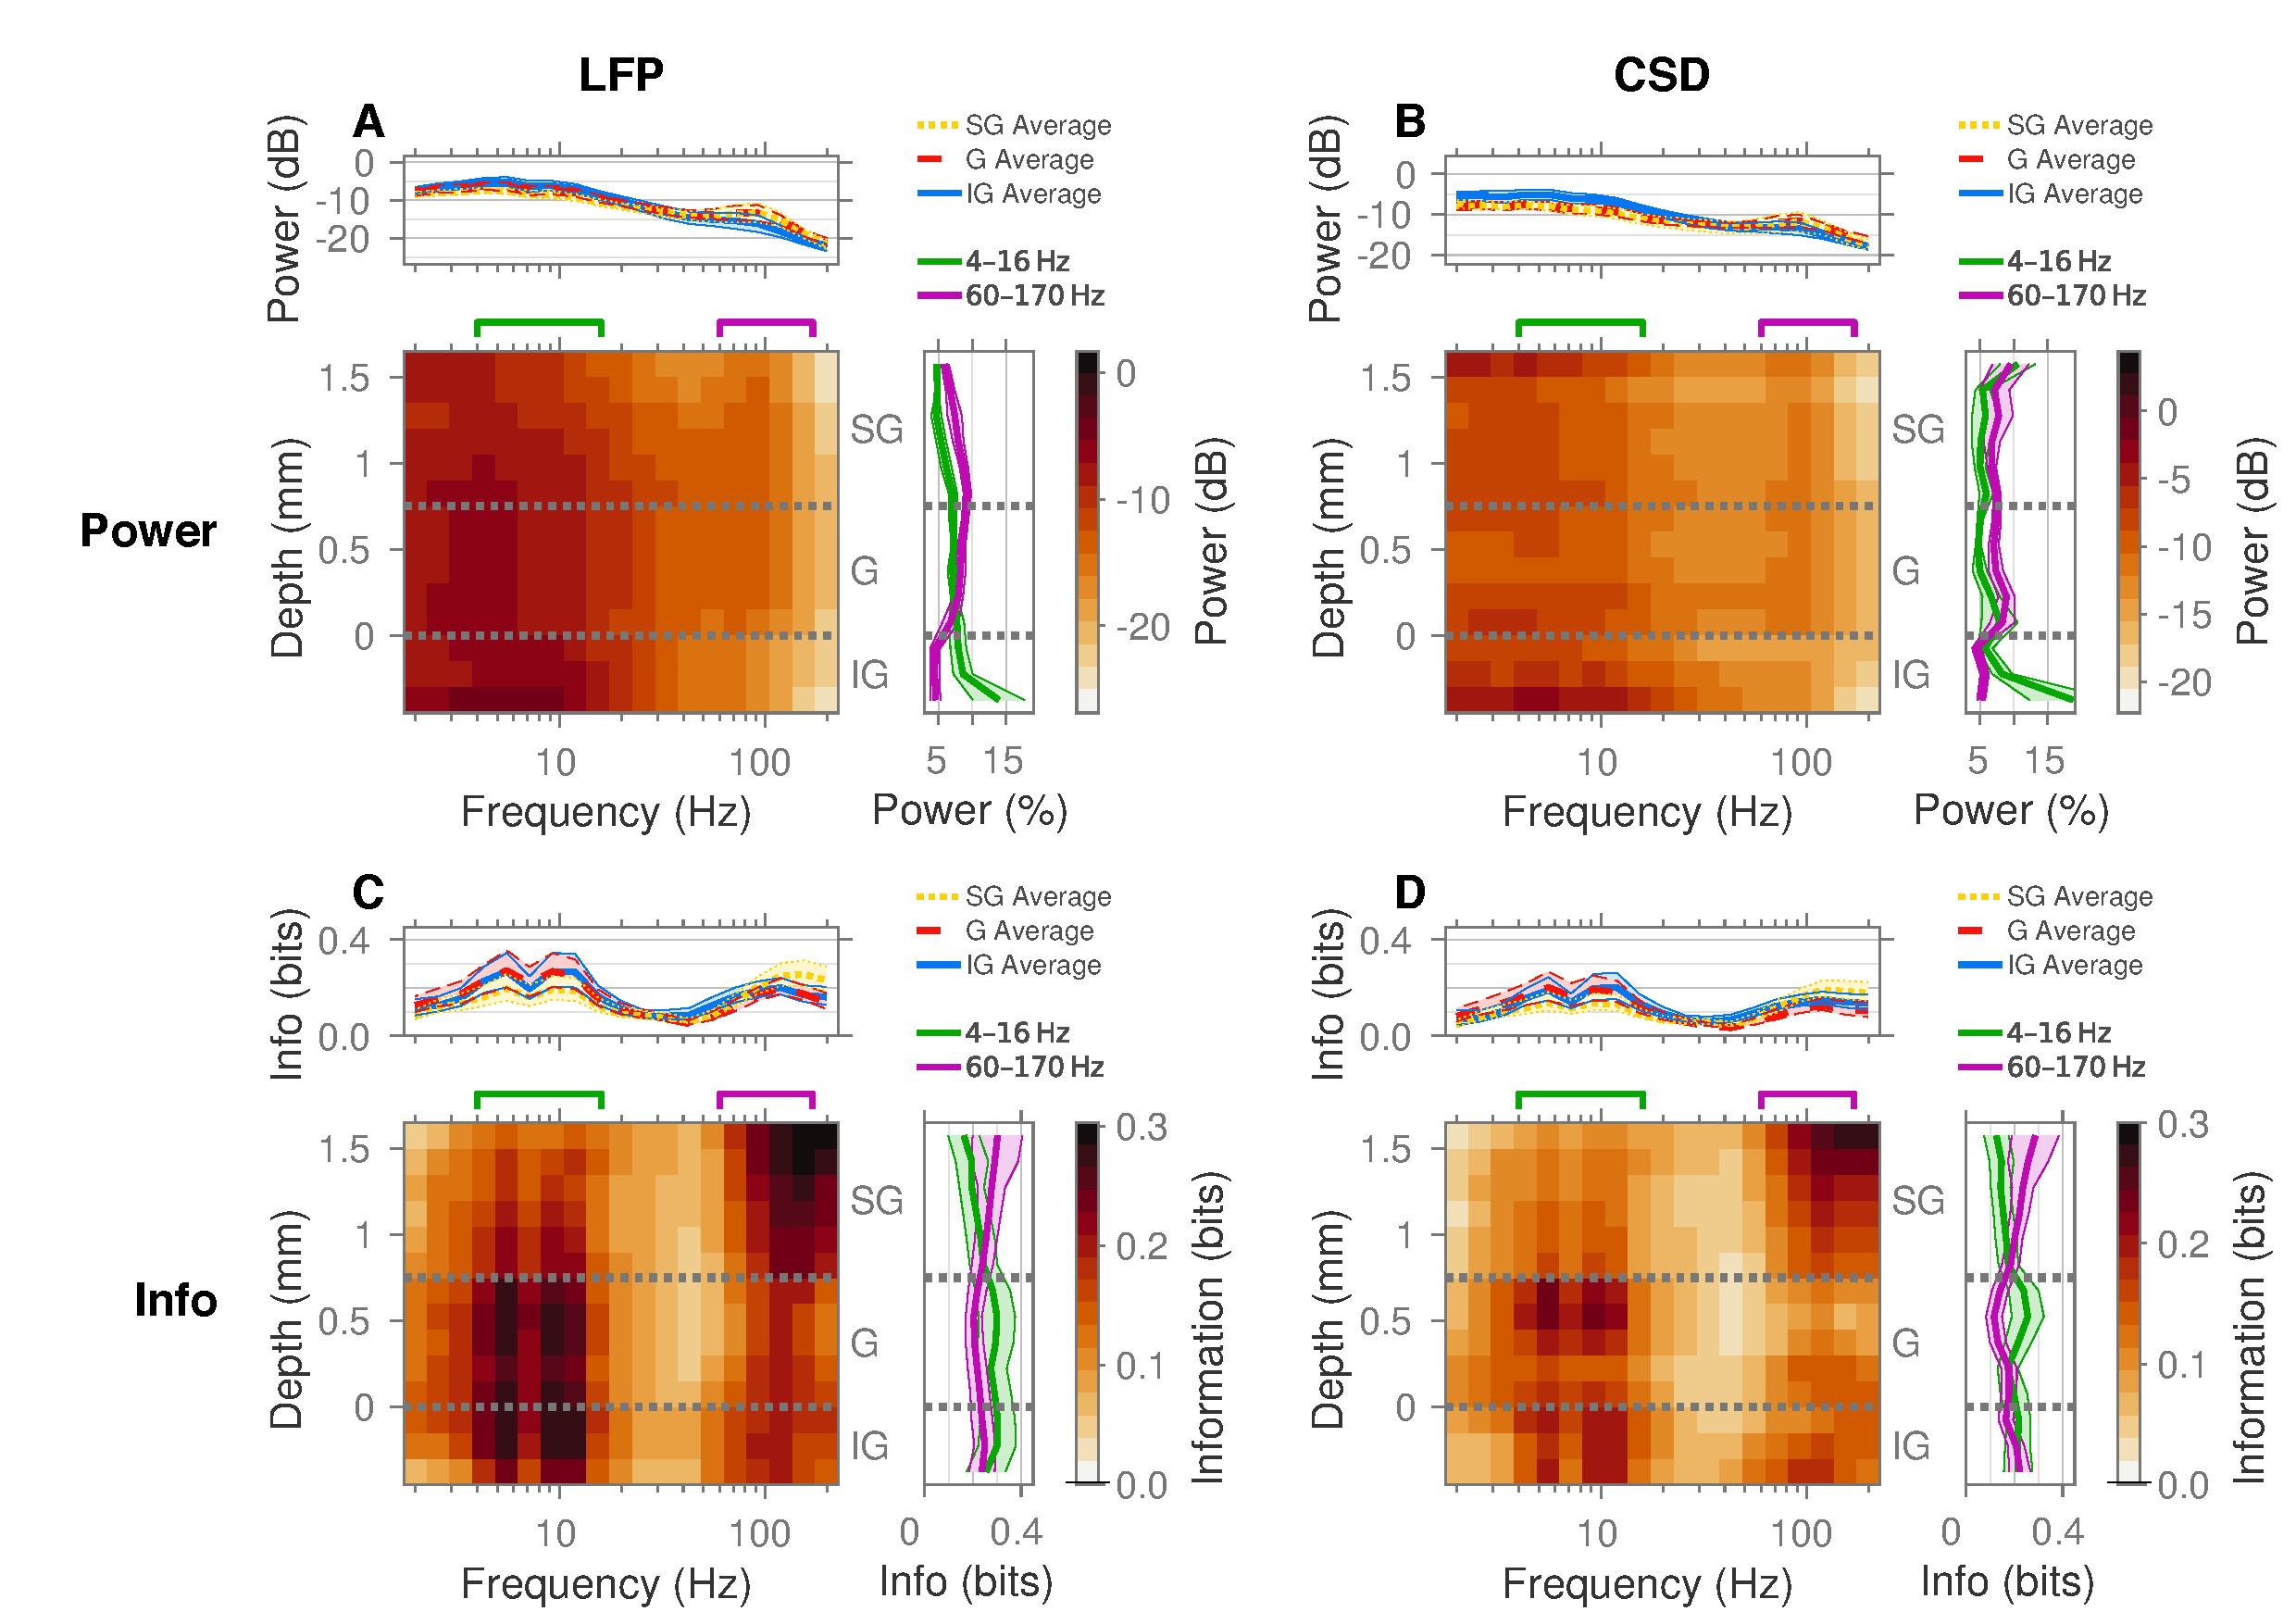
\includegraphics[width=\columnwidth]{fig2}
%
\caption{%
\textit{Distribution of visual stimulus information across both cortical depth 
and frequency.}
A: Distribution of \ac{LFP} power during stimulus presentation.
Plot shows the geometric mean 
power over 6 sessions.
Above, mean power within \ac{SG}, \ac{G} and \ac{IG} regions.
Right, laminar distribution of \ac{LFP} power in
\SIrange{4}{16}{Hz} and \SIrange{6}{170}{Hz} frequency bands.
B: Same as A, but distribution of \ac{CSD} power instead of \ac{LFP} power.
C: Distribution of information about the stimulus contained in \ac{LFP} power.
Plot 
shows the mean information over 6 sessions.
Above, mean information within \ac{SG}, \ac{G} 
and \ac{IG} regions.
Right, cortical distribution of information in the power in
\SIrange{4}{16}{Hz} and \SIrange{6}{170}{Hz} frequency bands.
D: Same as C, but for information in \ac{CSD} power instead of \ac{LFP} power.
Note that the information (C+D) is distributed very differently from the \ac{LFP} and \ac{CSD} power.}%
\label{fig:lam_2}
\end{figure}

We computed information about which frame is currently on screen in various frequency components of the \ac{LFP} and \ac{CSD} (see Experimental Methods).
Excluding boundary effects at the top and bottom of the cortex where white matter contaminates estimates, power is fairly smooth across depth and decays as frequency increases (Fig.~\ref{fig:lam_2}A-B).
However, the information contained in the power does not have such a smooth distribution and differs from this in both space and frequency domains.
Instead, information is contained in specific frequencies at specific depths, in a similar manner for \ac{LFP} and \ac{CSD} (Fig.~\ref{fig:lam_2}C--D), with prominent maxima in the \SIrange{4}{16}{Hz} range at the top of the \ac{G} region, and the \SIrange{60}{250}{Hz} range near the top of the \ac{SG} region.
Additionally, there are local maxima in \ac{IG} for both the \SIrange{4}{16}{Hz} and \SI{60}{250}{Hz} ranges.
These results are consistent across sessions (Sup Fig.~\ref{fig:lam_2}).
As the information in the \ac{CSD} has better spatial localisation than the \ac{LFP} (Einevoll, Kayser, Logothetis, \& Panzeri, 2013; Kajikawa \& Schroeder, 2011), for the remainder of the paper we study only the \ac{CSD}.

These findings suggest that there are different information channels in a single cortical column.

\subsection{Information redundancy between frequencies}
Having identified the most informative regions in depth and frequency, there are two possibilities: either these regions contain the same information about the stimulus, through transcoding of one frequency range to another across the cortex, or the regions contain different information about the stimulus.
We investigated how similar the information was by computing the redundancy of information contained in pairs of frequencies (see Experimental Methods).
We found there are two frequency domains within which information is redundant: \SIrange{4}{40}{Hz} and \SI{>40}{Hz} (Fig.~\ref{fig:lam_3}A).
Furthermore, the information contained in neural frequencies \SI{<40}{Hz} is different to the information contained in frequencies SI{>40}{Hz}, since these measured to be independent (redundancy \SI{<=0}{\percent}).
The same \SI{<40}{Hz} and \SI{>40}{Hz} division is observed for the signal correlation (Sup Fig.~\ref{fig:lam_3}), and our results corroborate earlier findings (Belitski et al., 2008).
Based on these and the above results, we extracted two bands (\SIrange{4}{16}{Hz} and \SIrange{60}{170}{Hz}) that contain the most information and independently encode information about the stimulus.

\begin{figure}[htbp]
\centering 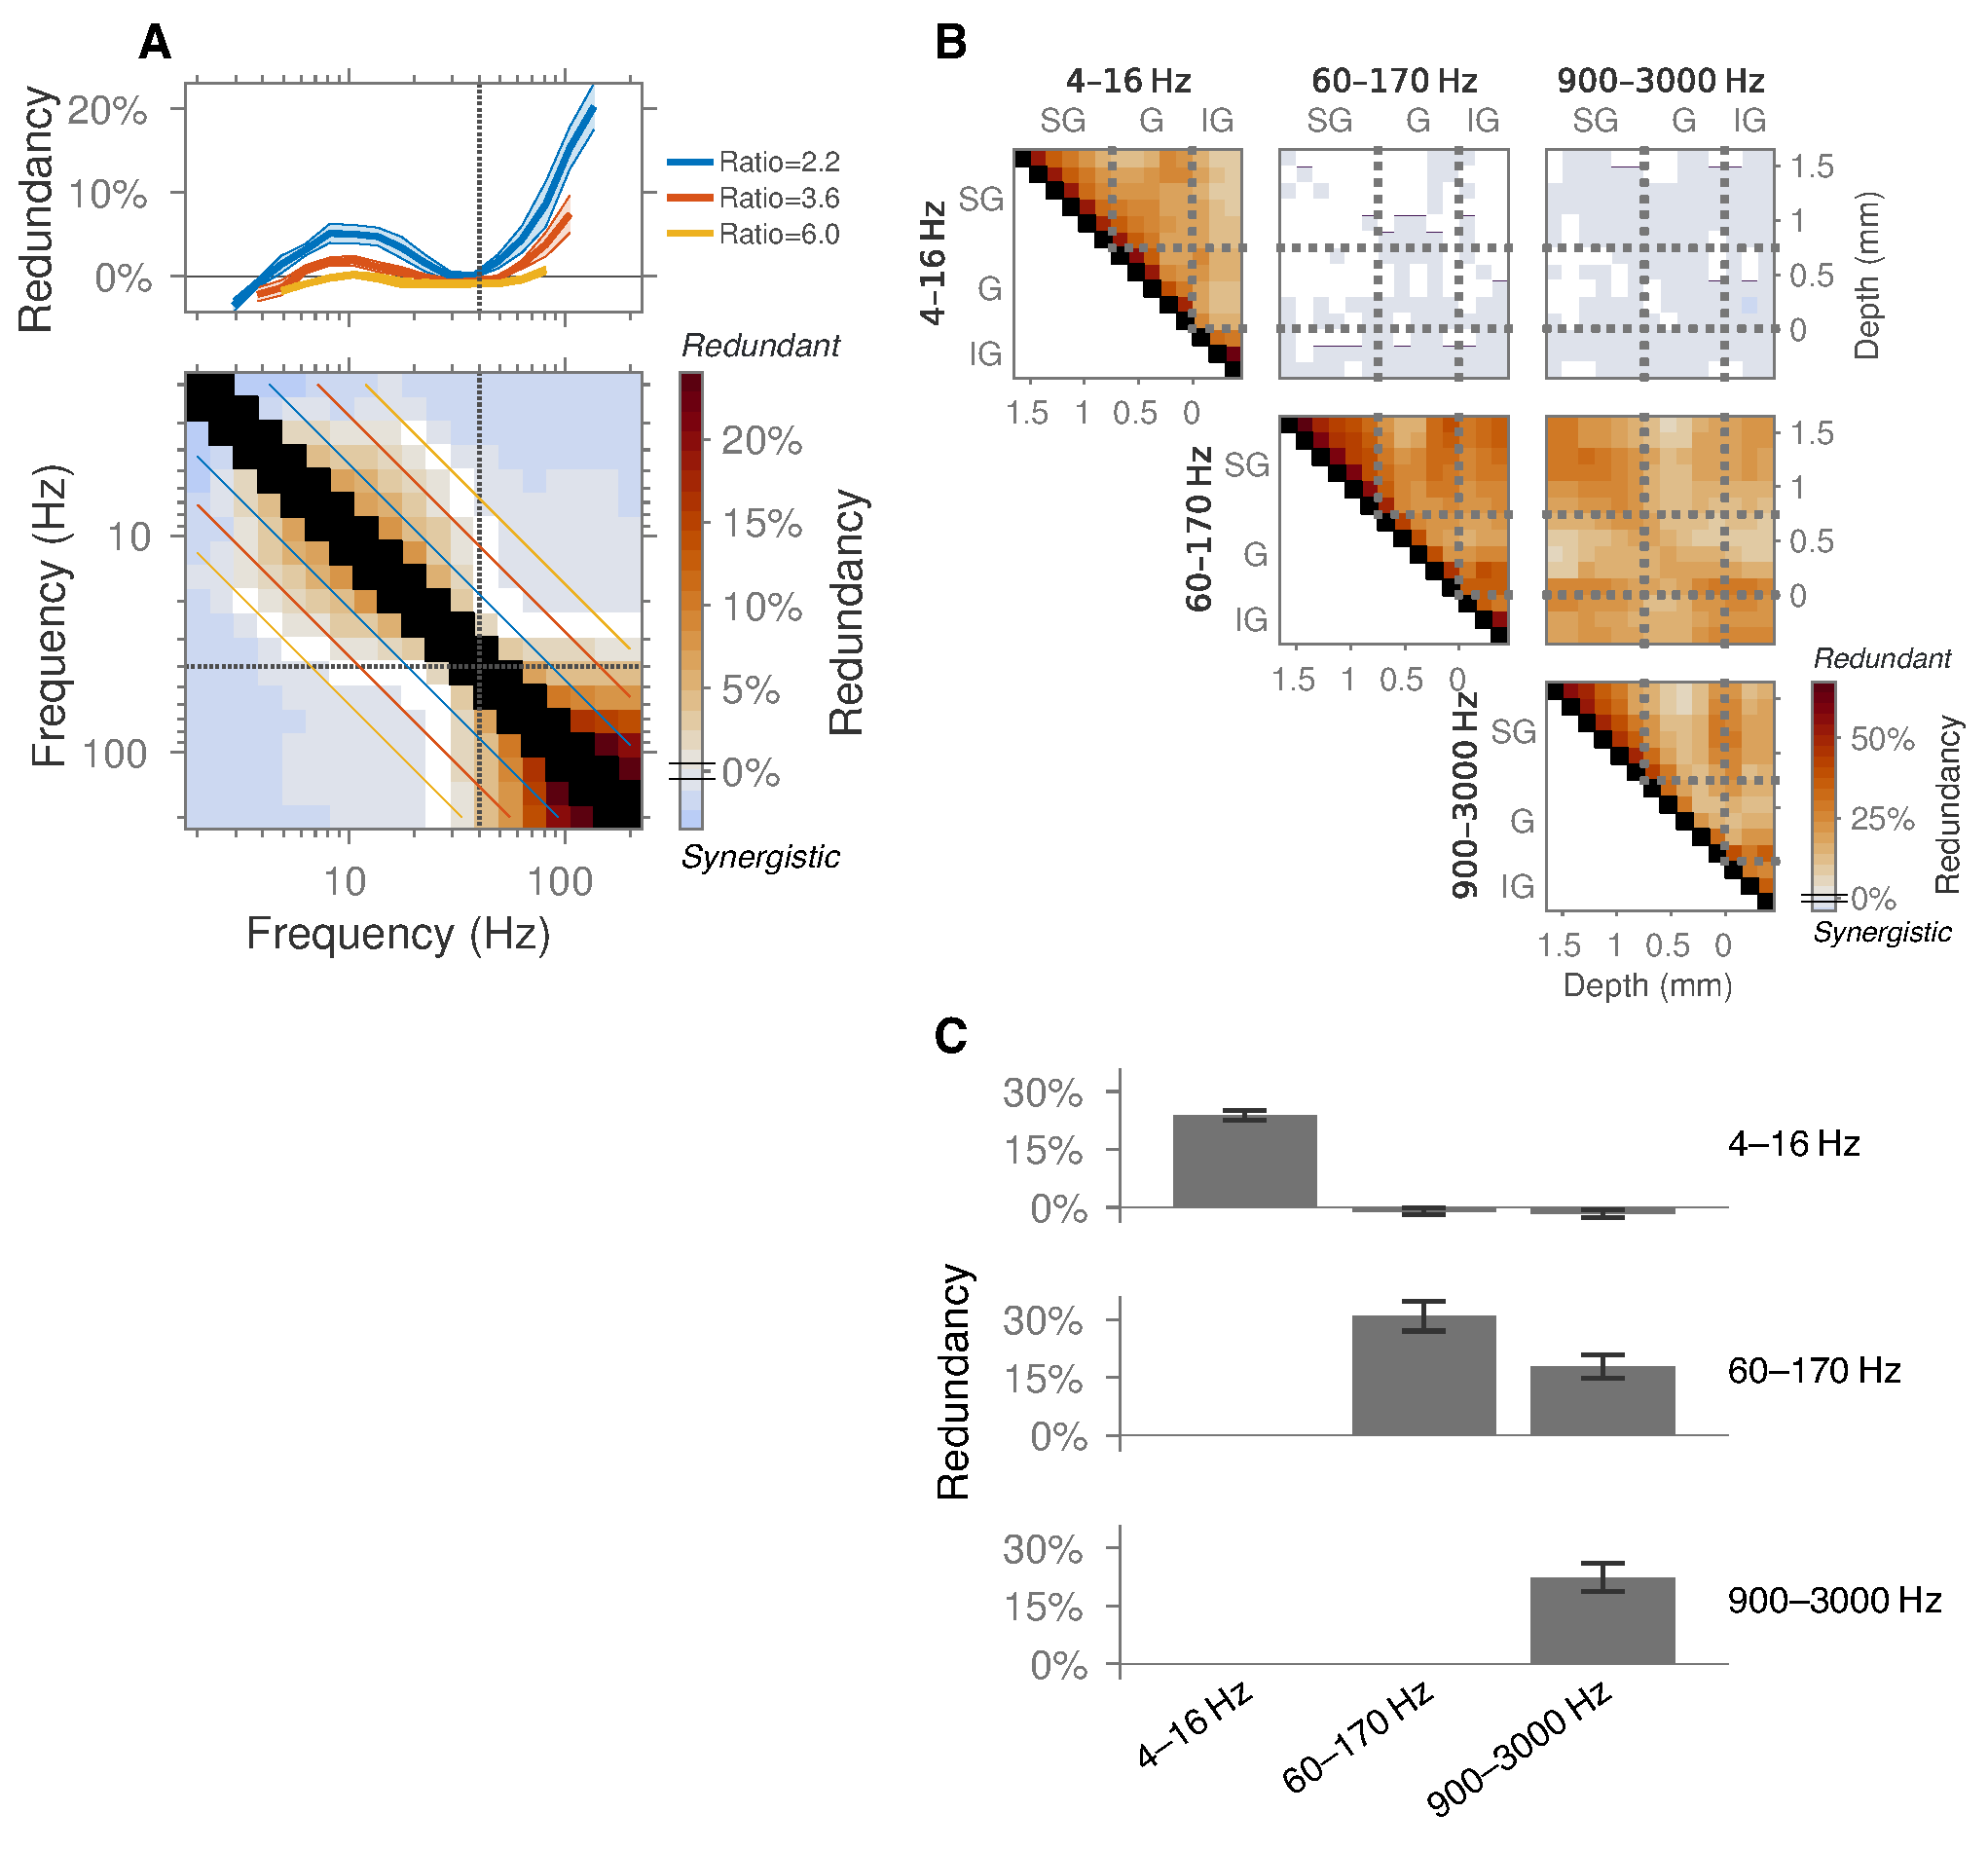
\includegraphics[width=\columnwidth]{fig3}
%
\caption{%
\textit{\ac{CSD} information redundancy across frequency bands and laminae.}
A: Median redundancy between pairs of frequencies over the 12 recording 
sites, averaged over 6 sessions.
B: Redundancy between pairs of recording sites of the information in three 
frequency bands.
Mean of 6 sessions.
C: Average of cross-channel redundancy shown in B.
Note, that while there is substantial redundancy within bands and between the 
\SIrange{60}{170}{Hz} and \SIrange{900}{3000}{Hz} bands, there is little redundancy between the \SIrange{4}{16}{Hz} and
\SIrange{6}{170}{Hz} band, indicating independent coding.}%
\label{fig:lam_3}
%
\end{figure}

\subsection{Information redundancy across depth}
Having established the independence of these bands, we investigated the redundancy between the power of oscillations at different cortical depths (Fig.~\ref{fig:lam_3}B).
For the \SIrange{4}{16}{Hz} frequency range, we found there is some redundancy across the entire cortical depth, but there are two distinct cortical regions (above and below the \ac{CSD} reversal, marked as 0mm depth) within which information is more redundant.
These findings are in agreement with (Maier, Adams, Aura, \& Leopold, 2010), who found a transition corresponding to the \ac{G}/\ac{IG} boundary which isolated two cortical regions with high coherence \SI{<100}{Hz}.

Gamma oscillations (\SIrange{6}{170}{Hz}) code, with substantial redundancy across the cortical depth, with some compartmentalisation of \ac{SG} and \ac{IG} activities.
In addition we also included the \ac{MUA} signal, which corresponds to the local population firing rate.
There is less redundancy of information across cortical depths for \ac{MUA} than for gamma; this observation is due to spiking activity being more localised than gamma oscillations.
In agreement with previous findings (Belitski et al., 2008), we find that information contained in the gamma range and information in the \ac{MUA} are redundant with each other.
This is to be expected, since \ac{MUA} is known to be correlated with the gamma cycle.(due to peaks/troughs in gamma relating to peaks/troughs in firing rate)

Overall redundancy is summarised in Fig.~\ref{fig:lam_3}C, which shows the average across all cortical depths for each pair of frequency bands.

Importantly, we find the information in the \SIrange{4}{16}{Hz} range is independent of the information contained in both gamma and \ac{MUA} frequency ranges across all cortical depths.
In particular, this means the two localised high information regions in depth-frequency space from Fig.~\ref{fig:lam_2}D contain independent information to one-another.
Importantly, this mean this argues against a situation where \ac{SG} contains the same information as \ac{G}/\ac{IG} activity transcoded from low-frequency to high-gamma oscillations; at least some of the information is unique to each.

\subsection{Information about spatial frequency components of visual stimulus}
In the above, we have seen there are two frequency bands in \ac{V1} which, across all the cortical depth, contain independent information to each other.
Next we investigate what aspects of the visual scene these two independent components contain.
Since neurons in the primary visual cortex are known to respond strongly to moving sinusoidal gratings with specific spatial frequencies, we considered how much information the frequency bands contained about changes in luminance as a function of spatial frequency.
Hereto, we decomposed the series of frames in the movie into set of spatial frequency components by finding the rate of change of luminance within a given set of spatial frequency bands (see Fig.~\ref{fig:lam_4}; Experimental Methods), and then computed the amount of information about this series contained in the neural activity.

\begin{figure}[htbp]
\centering 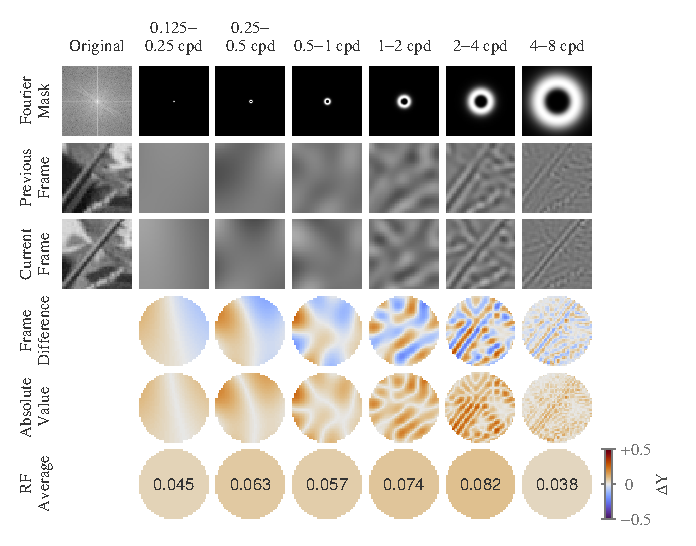
\includegraphics[width=\columnwidth]{fig4}
%
\caption{%
\textit{Extraction of spatially filtered luminance components.}
The luminance of the original video (left) is 
fast-Fourier transformed in a $224 \times 224$ px square for each frame (top-left: \ac{FFT} of 
``current frame'').
The mask isolates bands of spatial frequencies that are one octave wide (Row 1), yielding 
the spatially filtered frames (Rows 2 and 3).
The stimulus magnitude at each spatial frequency band was obtained 
by taking the luminance difference of successive frames (Row 4), 
taking its absolute value (Row 5), 
and averaging this within the receptive field (Row 6).
%This provides us with a temporal sequence of the rate of change of luminance for 
%each spatial resolution.
}%
\label{fig:lam_4}
%
\end{figure}

\begin{figure}[htbp]
\centering 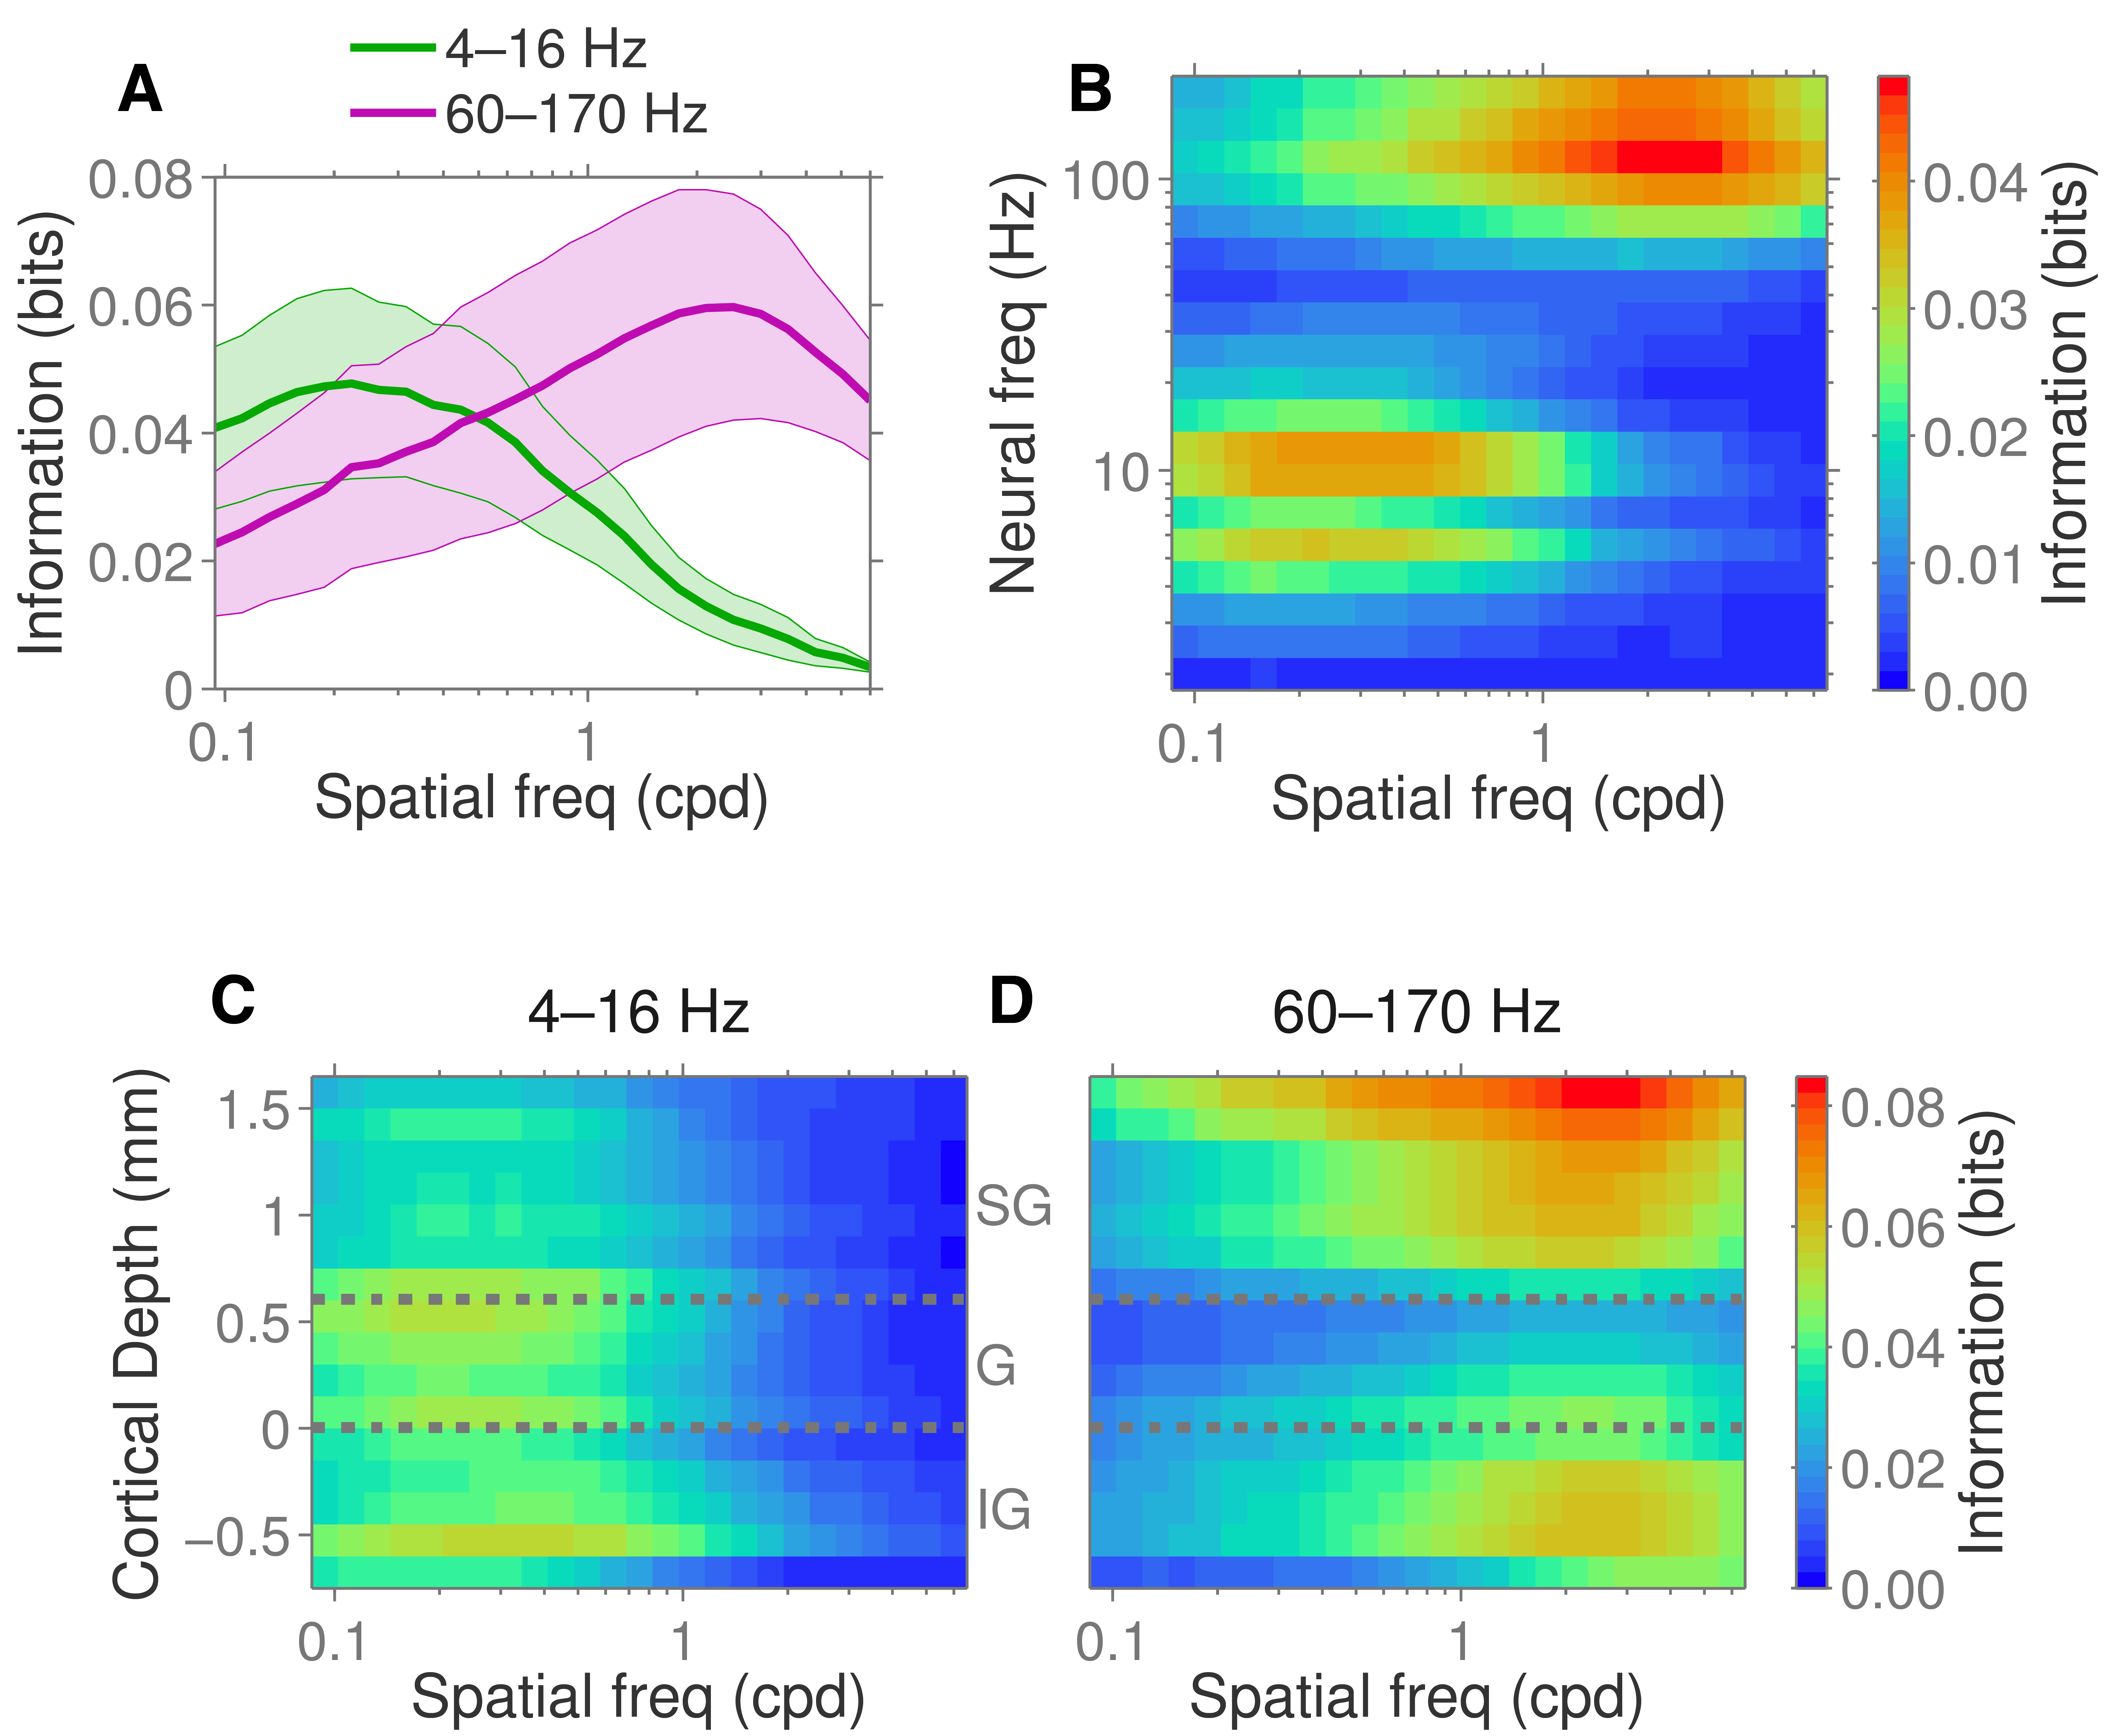
\includegraphics[width=\columnwidth]{fig5}
%
\caption{%
\textit{Information about different spatial components across laminae and frequency bands.}
A: Information about spatial components of the stimulus contained in 
low frequency \ac{CSD} power (\SIrange{4}{16}{Hz}, average of information within \ac{G} region; green) and high 
frequency \ac{CSD} power (\SIrange{6}{170}{Hz}, average of information within \ac{SG} region; purple).
Shaded region: standard error across 6 sessions.
B: Information about visual spatial components contained in a range of \ac{CSD} frequencies, median over 12 recording sites.
C,D: Information in low (\SIrange{4}{16}{Hz}) and high (\SIrange{6}{170}{Hz}) 
\ac{CSD} frequency bands across cortical laminae.
Plots A-D are mean of 6 sessions.}%
\label{fig:lam_5}
%
\end{figure}

We found the low frequency \ac{CSD} bands (\SI{<40}{Hz}) contained more information about low, coarse spatial frequencies (\SIrange{0.1}{0.6}{\cpd}), whereas the higher frequencies (\SI{>40}{Hz}) contained more information about high, fine spatial frequencies (\SIrange{0.6}{5.0}{\cpd}) (Fig.~\ref{fig:lam_5}B).
This was not a continuous transition; instead we observe an abrupt change at \SI{40}{Hz}, with lower and higher neural oscillation frequencies tuned to stimulus features with different spatial frequencies.
This was true across the entire cortical depth (Fig.~\ref{fig:lam_5}C--D), where the two frequency bands (\SIrange{4}{16}{Hz} and \SIrange{60}{170}{Hz}) contained information about opposing spatial frequencies.
The distribution of information across the cortical depth corresponds to that found in Fig.~\ref{fig:lam_2}D.
These results are summarised in Fig.~\ref{fig:lam_5}A, which shows the average across the cortical depth.
Information reaches its maxima around \SI{0.2}{\cpd} for the \SIrange{4}{16}{Hz} frequency range and \SI{2.5}{\cpd} for the \SIrange{60}{170}{Hz} frequency range.

In Fig.~\ref{fig:lam_6}, we summarise the previous results by extracting two spatial frequency bands: coarse (\SI{<0.3}{\cpd}, low-pass spatial filter) and fine (\SI{>1}{\cpd}, high-pass spatial filter), example traces for which are shown above Fig.~\ref{fig:lam_6}A.
These spatial components have low correlation between them (Fig.~\ref{fig:lam_6}B; $r=0.18$).
Example \ac{CSD} traces are also shown for two electrode contacts over same time period (left side).
Note that peaks and troughs in the coarse luminance signal are coincident with peaks and troughs with the alpha power, and similarly for the fine luminance and gamma power, indicating the positive relationship between stimulus and cortical response.
This observation is quantified by the correlation and mutual information between these components (Fig.~\ref{fig:lam_6}A).

\begin{figure}[htbp]
\centering 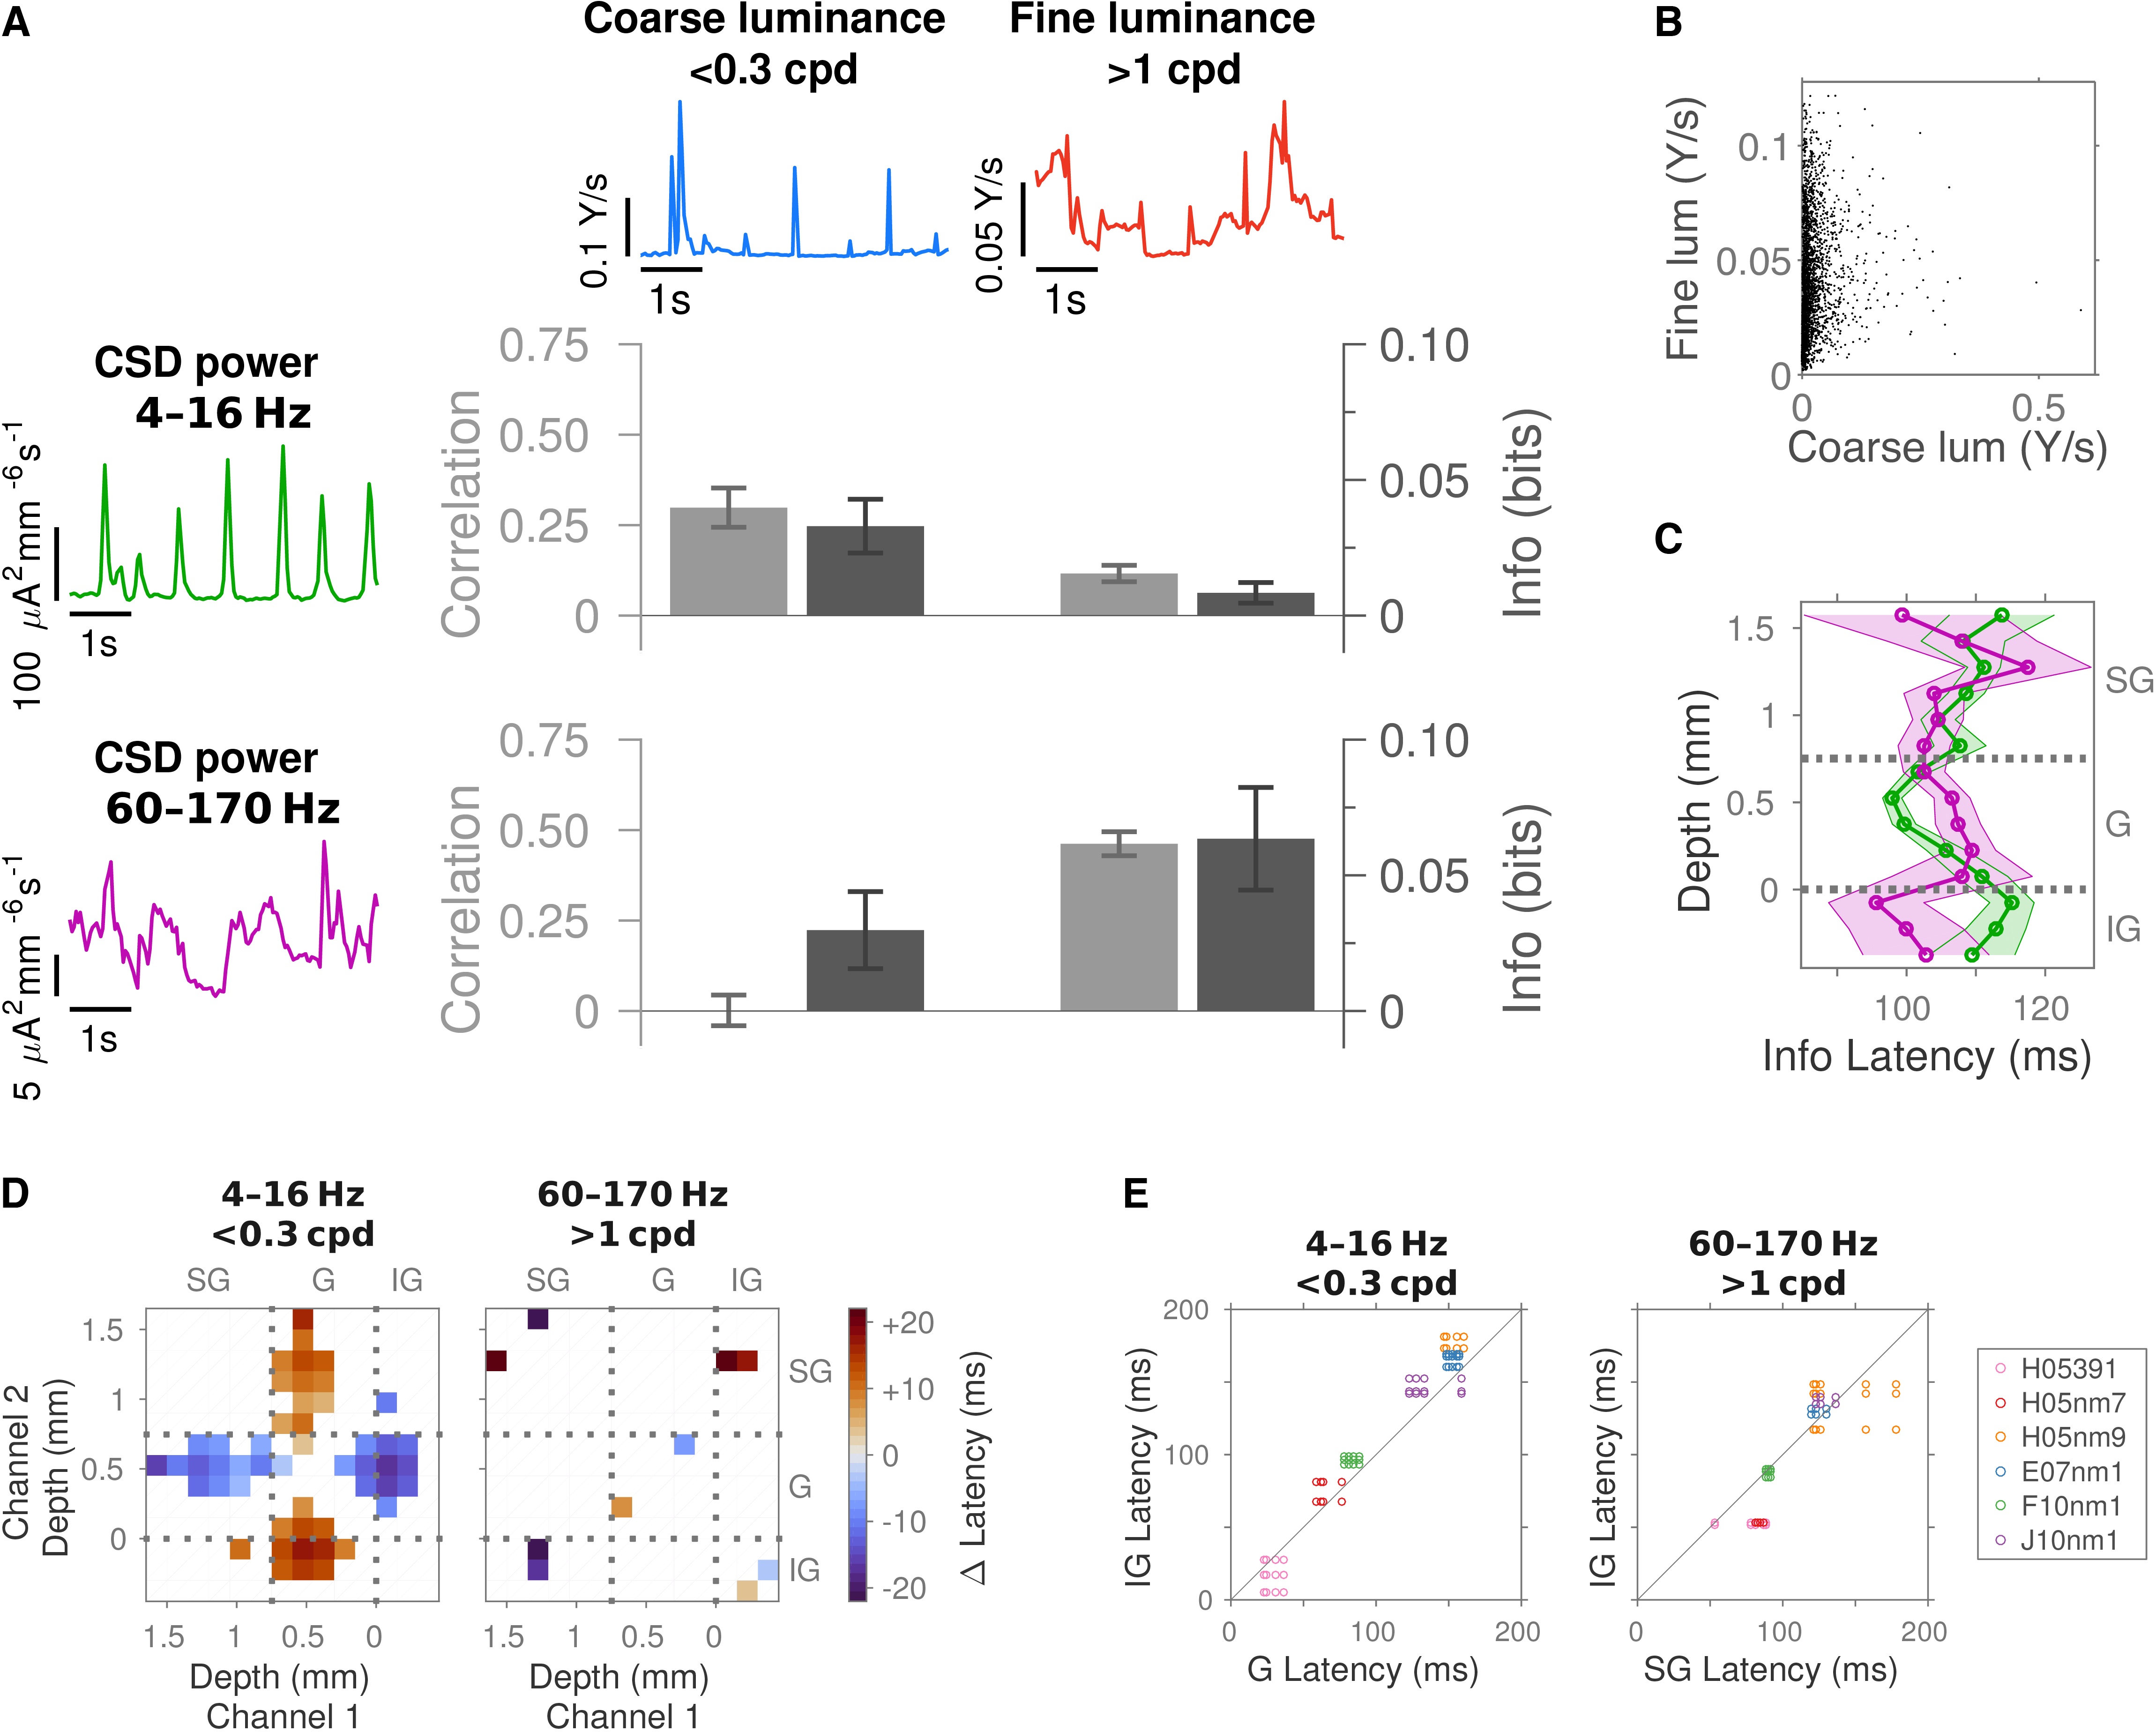
\includegraphics[width=\columnwidth]{fig6}
%
\caption{%
\textit{Overview of information components.}
A: Relationship between Coarse/Fine changes in luminance and Low/High frequency neural activity.
Left: Instantaneous power in \SIrange{4}{16}{Hz} band (averaged over trials and \ac{SG} layers) and \SIrange{6}{170}{Hz} band (averaged over trials and \ac{G} layers) for an example session (H05nm7).
Above: Coarse (\SI{<0.3}{\cpd}) and fine (\SI{>1}{\cpd}) rate of change in luminance over the same time period.
The barchart shows, for each pair of stimulus and response, Pearson's correlation coefficient (pale grey; left-hand axis) and mutual information (dark grey; right-hand axis).
B: Fine versus coarse change in luminance for each frame change in the stimulus.
C: Lag between stimulus and response yielding maximal information (green: \SIrange{4}{16}{Hz} and coarse luminance; purple: \SIrange{6}{170}{Hz} and fine luminance).}%
\label{fig:lam_6}
%
\end{figure}

\subsection{Layer 1 \SIrange{6}{170}{Hz} amplitude is coupled to L5 \SIrange{4}{16}{Hz} phase}
In previous section ``Information redundancy across depth'', we showed that high and low \ac{LFP} frequencies contain independent information to one-another.
To further investigate the relationship between these two bands, we computed the cross-frequency coupling between the low frequency phase and high frequency oscillation amplitude.
In agreement with previous work (Spaak, Bonnefond, Maier, Leopold, \& Jensen, 2012), we found there is significant coupling between the \SIrange{4}{16}{Hz} phase in lower-\ac{G} and mid-\ac{IG} with the and amplitude of \SIrange{6}{170}{Hz} oscillations in upper \ac{SG} (Fig.~\ref{fig:lam_8}).
There is also localised coupling between the \SIrange{4}{16}{Hz} phase with \SIrange{6}{170}{Hz} amplitude in \ac{G} and \ac{IG}.
These findings were all true of both the stimulus driven and spontaneous recordings.

\begin{figure}[htbp]
\centering 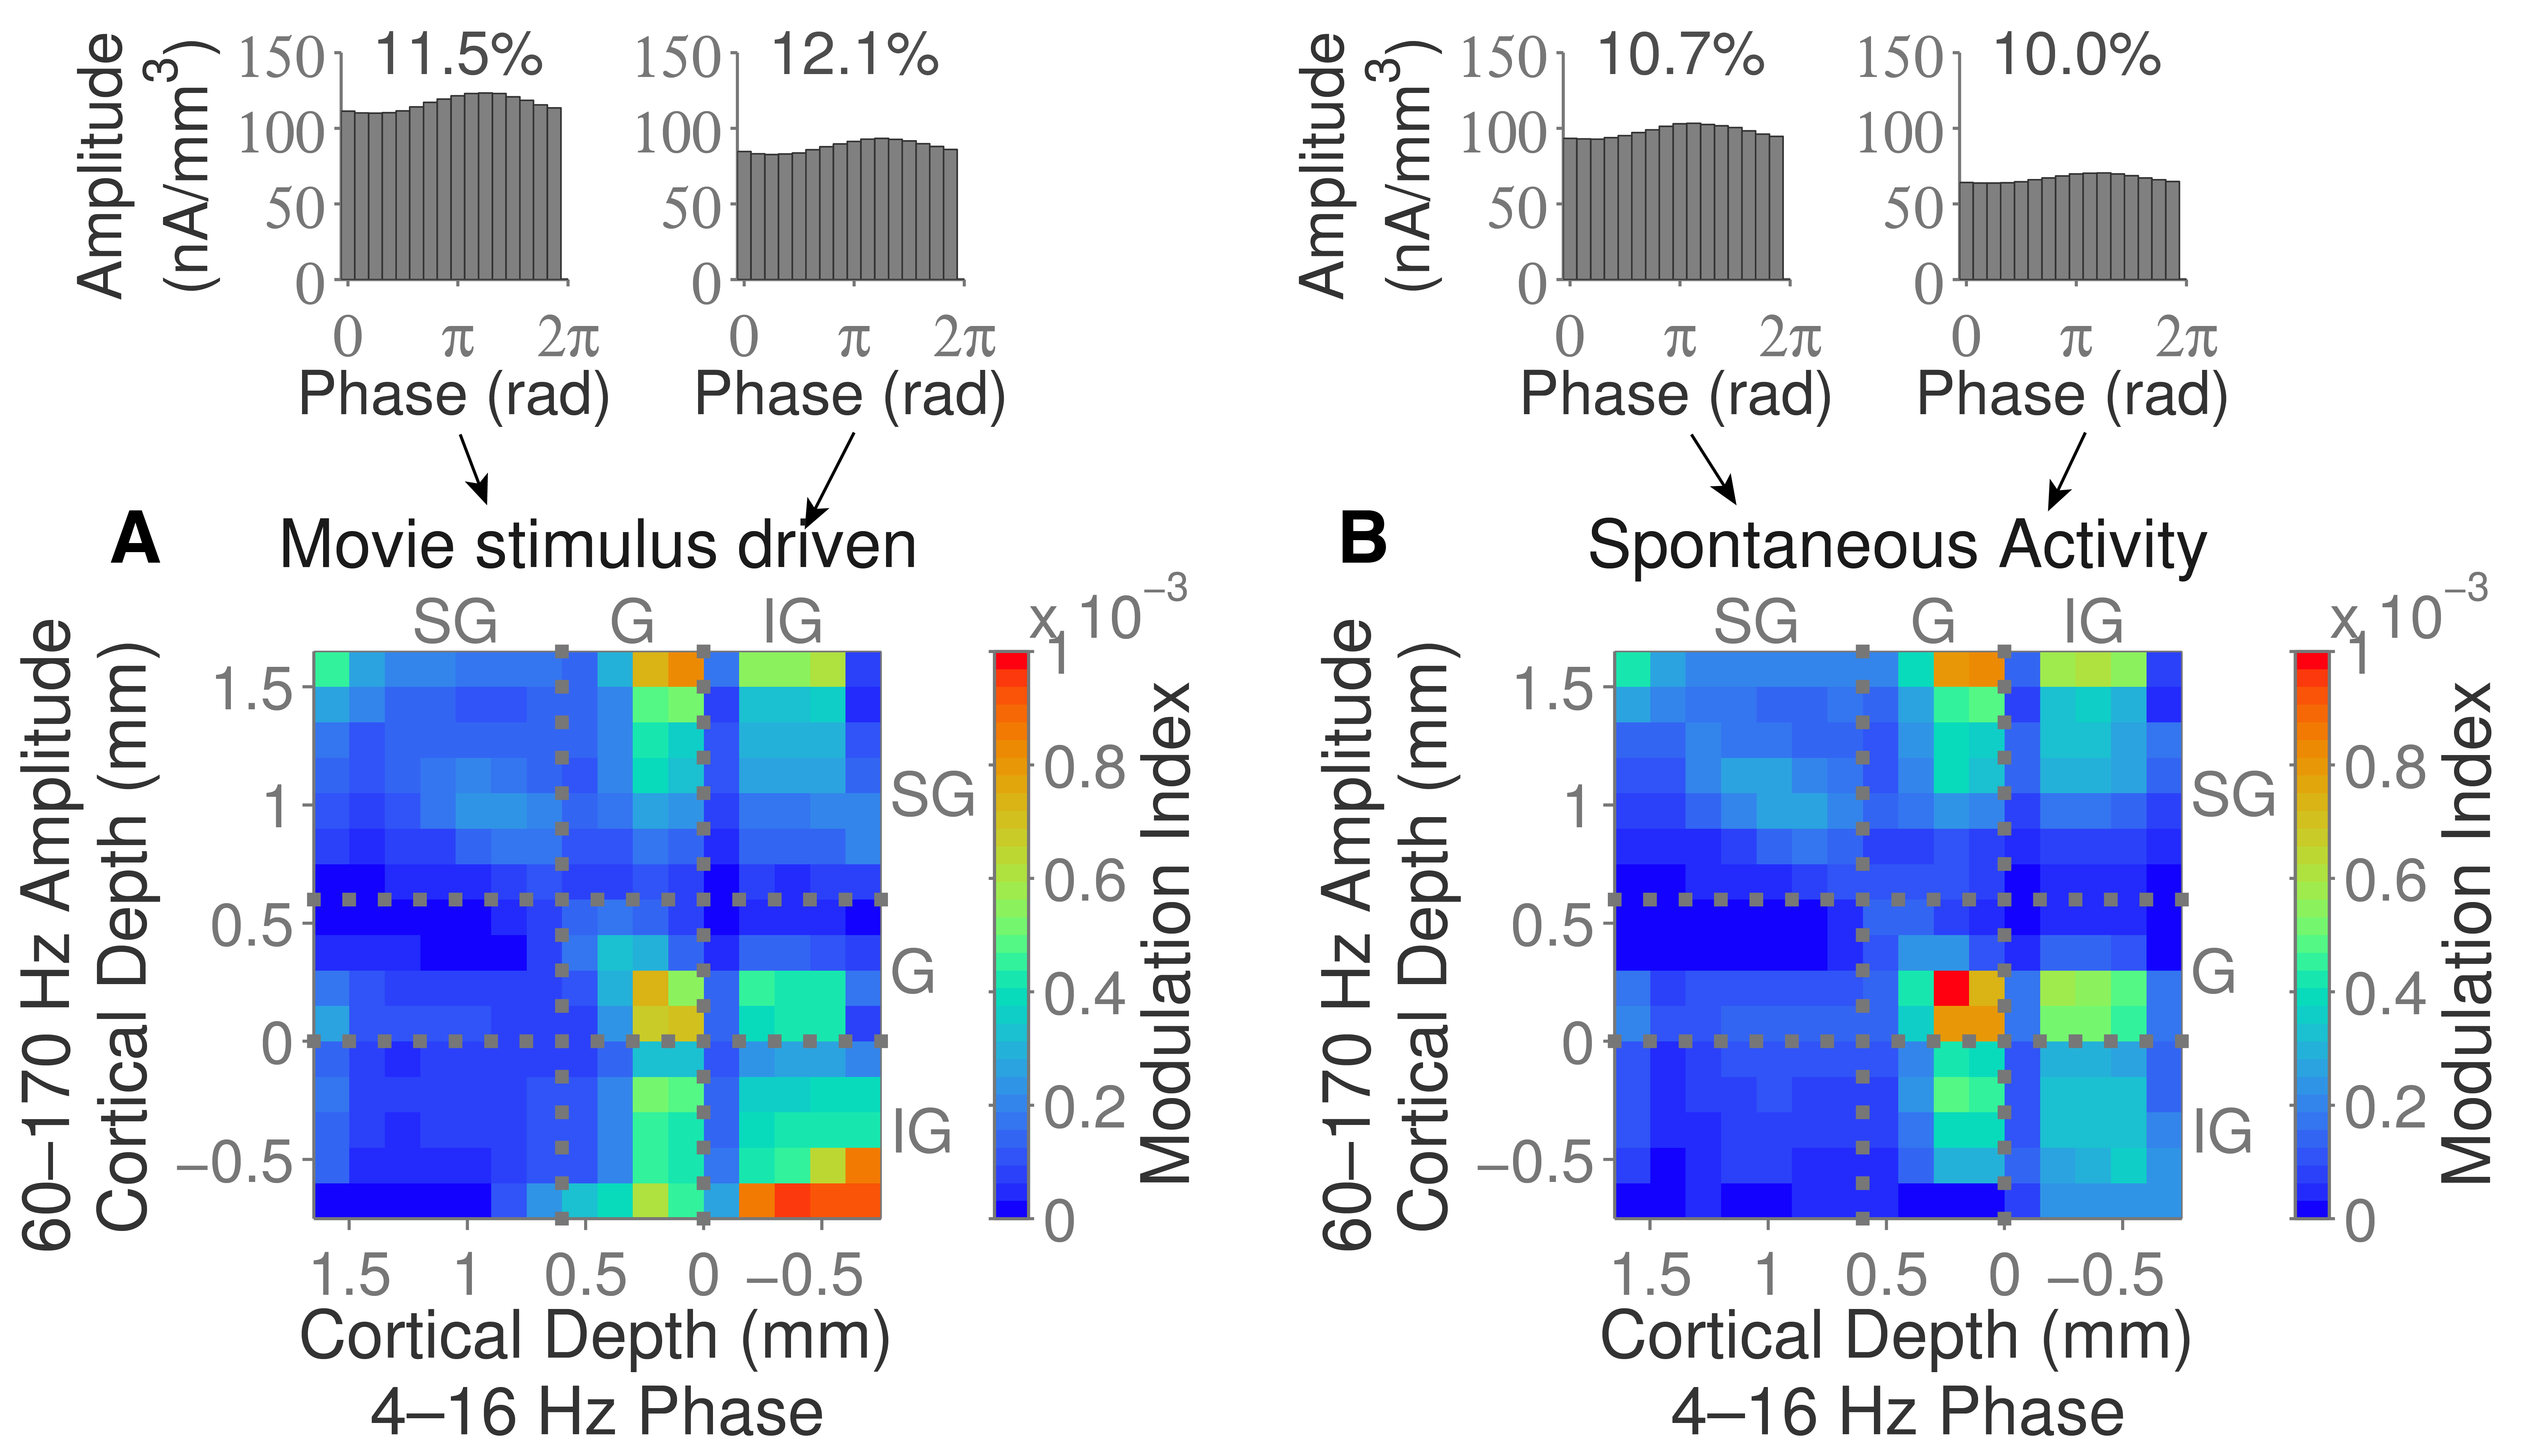
\includegraphics[width=\columnwidth]{fig8}
%
\caption{%
\textit{Cross-frequency phase-amplitude coupling}
Phase-amplitude modulation index between low frequency (\SIrange{4}{16}{Hz}) phase and high 
frequency (\SIrange{6}{170}{Hz}) amplitude (A: movie driven activity; B: spontaneous 
activity).
Mean of 5 sessions.
Above, amplitude as a function of binned phase for an example session (H05391).
Left inset: \ac{IG}/\ac{IG} coupling; Right inset: \ac{IG}/\ac{SG} coupling.}%
\label{fig:lam_8}
%
\end{figure}

%-------------------------------------------------------------------------------
\section{Discussion}
In summary, we find while \ac{LFP} power is smooth and its depth profile is close to flat (Fig.~\ref{fig:lam_2}a,b) the information that the \ac{LFP} encodes reveals much more structure.
We found there are two cortical regions at which oscillations in these frequency ranges are much more informative.
Namely \SIrange{4}{16}{Hz} at upper granular and mid-infragranular, and \SIrange{6}{170}{Hz} at upper supragranular and mid{}-infragranular regions.Previous work (Belitski et al., 2008) has shown that in the macaque primary visual cortex information is coded in two frequency bands (\SI{<40}{Hz} and \SI{>40}{Hz}) containing independent information about natural visual scenes.
Our analysis extended across the cortical depth, and we found there are two cortical regions at which oscillations in these frequency ranges are much more informative (\SIrange{4}{16}{Hz} at upper-\ac{G} and mid-\ac{IG}; \SIrange{6}{170}{Hz} at upper-\ac{SG} and mid-\ac{IG} regions).

We also examined whether changes in luminance at different spatial frequencies induced differential changes in the cortex as a function of neural frequency and depth.
Namely, high spatial frequencies are encoded in oscillations faster than \SI{40}{Hz} and low spatial frequencies are encoded in oscillations slower than \SI{40}{Hz}.
We found that frequencies below and above \SI{40}{Hz} contain information about different spatial frequencies.

There are multiple possible interpretations of these findings, of which one, many, or even none may be correct.
Firstly, it is conceivable that the coding of different aspects of the stimulus into different frequency bands is a computational strategy of the cortex.
Our results suggest there is multiplexing in the cortex, with low frequency and high frequency oscillations of the same population activity simultaneously encoding low and high spatial frequency components of the stimulus respectively.
The idea of different frequency bands conveying different spatial frequency components of the stimulus has been proposed before from the results of an \ac{EEG} study (Smith, Gosselin, \& Schyns, 2006).

One would expect that if certain oscillation frequencies in the visual cortex contain information about specific aspects of the stimulus, this is likely to be because the brain has encoded this information into oscillations in the activity of the local population.
This would only make sense if the information is utilized by the brain in order to interpret its stimuli.
Consequently, our results indicate there is multiplexing in the cortex, with low frequency and high frequency oscillations of the same population activity simultaneously encoding low and high spatial frequency components of the stimulus respectively.
Intuitively, information contained in the two frequency bands can be combined by downstream visual cortical regions to regain the original stimulus as necessary.
The idea of different frequency bands conveying different spatial frequency components of the stimulus has been proposed before from the results of an \ac{EEG} study (Smith, Gosselin, \& Schyns, 2006).

Additionally, we can speculate about why separating the visual scene into low frequency (coarse) and high frequency (fine) components in \ac{V1} is useful.
One possibility is that low frequency oscillations are output from \ac{V1} along the dorsal visual stream, whereas high frequency oscillations travel propagate through the ventral stream.
Another possibility is that broad, coarse changes in the stimulus are useful for making rapid responses in the motor cortex to sudden changes, such as approaching threats.

Separation into low and high frequency domains with different properties seems to be a common property of the cortex.
In motor cortex, activity at \SI{<13}{Hz} and \SI{>60}{Hz} relates to behaviour but there is a separating band \SI{\approx30}{Hz} which does not (Rickert et al., 2005).
In the hippocampus, there is a gating effect between \SI{30}{Hz} and \SI{40}{Hz}, with lower but not higher frequencies able to propagate to the cortex (Moreno, Morris, \& Canals, 2015).
[also some unpublished research by Julian Hoffman into independent oscillations in the barrel cortex].
This suggests this encoding scheme is common across the cortex.
Some studies have suggested that the coupling of oscillations between two cortical regions facilitates the transmission between them.

A separation of visual stimuli into coarse and fine channels is known to occur before the stimuli arrive in the cortex.
The outputs from different types of \acp{RGC} travel to the cortex through different regions of \iac{LGN}.
The M-pathway arises from \acp{RGC} with large, achromatic receptive fields, and projects mainly onto layer 4C$\alpha$ in \ac{V1}.
The P-pathway originates with \acp{RGC} with smaller, chromatic \acp{RF} providing higher spatial resolution but lower temporal resolution; this pathway projects onto layer 4C$\beta$ (E M Callaway, 1998).
It is possible that the two frequency channels in \ac{V1} relate to the two pathways providing its inputs..
[Cite Nathaniel J Killian from AREADNE on information in low-frequencies of \ac{LGN}.
Nothing available to actually cite?]

Since \ac{L4} is generally regarded as the primary layer of \ac{V1} which receives afferent inputs from \iac{LGN}, some readers might wonder how information in the gamma band has ``arisen'' in \ac{SG} layers without passing through \ac{G}.
However, our results do not necessitate this.
Fine-resolution information about the visual stimulus can arrive from the \ac{LGN} into \ac{L4} of \ac{V1}, with the information encoded into which neurons the afferent connections target.
This information is not detectable from the population level activity.


As many readers will be aware, it has long been known that neurons in the primary visual cortex have a response curve tuned to a preferred spatial frequency.
Work demonstrating the spatial frequency preference of single neurons typically involves the presentation of moving sinusoidal grating with a particular spatial frequency.
[NOT SURE WHERE I WAS GOING WITH THIS{\dots}]

The higher frequency band contains information about higher spatial frequencies changes in the stimulus.
This corresponds to the detection of edges and texture, which are properties that single neurons in \ac{V1} are known to be selective for.


We observed that each frequency has a similar amount of power across the cortical depth, but oscillations at these frequency ranges contain much more information at particular cortical depths.
This is curious as it indicates that, for any given frequency band, oscillations are present in all cortical depths, but most of the oscillations exhibited are not stimulus encoding.
This seems wasteful.
[important point]

We observed qualitatively that information-carrying events in \ac{L4} were large, temporary deflections with a long duration (low frequency), whereas \acs{L5}/6 contained sustained oscillations (see Fig.~\ref{fig:lam_1}A for examples).
The deflections in \ac{L4} were usually coincident with scene cuts or rapid changes in the stimulus.
This could be interpreted as an error signal, since sudden, large changes in the stimulus would result in any predictive model of the stimulus making large errors.
However, a more simple interpretation is these deflections correspond to changes in the afferent input to \ac{V1} from \ac{LGN}.
In support of this, we note that the spatial scale of the information in the low frequency band (\SI{0.25}{\cpd}) approximately corresponds to the size of receptive fields for regions of the \ac{V1} corresponding to the parafovea (\SI{2}{\degree}).

The sustained oscillations in \acs{L5}/6 also contain information about coarse changes in the stimuli.
These cortical layers are known to have connections to the motor cortex, feedback to \iac{LGN} and receiving feedback from higher cortical regions.


Recent work has indicated that alpha and gamma bands are important for feedback and feedforward activity respectively (van Keroerle et al., 2014).
This study (van Keroerle et al., 2014) found that gamma waves are initiated at \ac{L4} and propagate outwards to the top of \ac{SG} and bottom of \ac{IG}, with alpha waves propagating in the opposite direction.
Our study finds the most information in gamma bands at the very top (and very bottom) of the cortex, and the most information in alpha bands at the top of \ac{L4} (and \ac{L6}).
Reconciling these results together, we find that there is most information in the power of the alpha and gamma oscillations at the cortical depths where they terminate, and the least where they originate.
This suggests that the oscillations are generated at one cortical depth without much stimulus dependency, but as the oscillations propagate up and down the cortex they are either amplified or supressed in a stimulus dependent manner.

In agreement with previous work (Spaak et al., 2012), we found there was cross-frequency coupling between the stimulus-encoding power of gamma oscillations in \ac{L1} and the phase of alpha oscillations in lower \ac{L4}.
Anatomically, we believe this is related to the pyramidal cell bodies in \ac{L5A}, which have apical dendritic tufts in \ac{L1} (Hill, Jia, Sakmann, \& Konnerth, 2013; Zhu \& Zhu, 2004).
This cross-frequency coupling could be one mechanism through which the \ac{L1} gamma wave containing high levels of information about the stimulus is converted into an alpha oscillation for feedback into the hierarchically lower cortical region.
Neurons in \ac{L5} are known to be related to long-range cortical output (Hill et al., 2013).


%-------------------------------------------------------------------------------
%\section{Supplementary Materials}
%
% \begin{flushleft}
% \tablefirsthead{}
% \tablehead{}
% \tabletail{}
% \tablelasttail{}
% \begin{supertabular}{m{1.6789999cm}|m{1.888cm}|m{2.3009999cm}|m{3.5479999cm}|m{5.303cm}}
% Session &
% Display &
% Video frame rate (fps) &
% Artefact Frequencies Removed (Hz) &
% Size of \SI{1}{\degree} square in visual field (in raw video pixels)\\\hline
% H05391 &
% Projector &
% \raggedleft 30.015 &
% 30 &
% 16.0 x 16.0 px\\
% H05nm7 &
% Projector &
% \raggedleft 30.015 &
% 30, 60 &
% 21.3 x 21.3 px\\
% H05nm9 &
% CRT &
% \raggedleft 118.098 &
% ~
%  &
% 17.8 x 17.9 px\\
% E07nm1 &
% CRT &
% \raggedleft 118.098 &
% 50, 150 &
% 17.9 x 17.8 px\\
% F10nm1 &
% Projector &
% \raggedleft 30.015 &
% 30, 60 &
% 21.3 x 21.3 px\\
% J10nm1 &
% CRT &
% \raggedleft 118.098 &
% ~
%  &
% 17.8 x 17.9 px\\
% \end{supertabular}
% \end{flushleft}
